\documentclass[a4paper, 12pt]{article}

\usepackage[top=1.5cm]{geometry}
\usepackage{mathtools}
\usepackage{graphicx}
\graphicspath{ {../Images/} }
\usepackage[utf8]{inputenc}
\usepackage[T1]{fontenc}
\usepackage{textcomp}
\usepackage{amssymb}
\usepackage{newtxmath}
\usepackage{ebgaramond}
\usepackage{amsmath, amssymb}
\usepackage{amsthm}


\newtheorem{theorem}{Theorem}

\theoremstyle{definition}
\newtheorem{problem}{Problem}

\theoremstyle{definition}
\newtheorem{example}{Example} 

\theoremstyle{definition}
\newtheorem{definition}{Definition}

\newtheorem{lemma}{Lemma}
\newtheorem{pro}{Proof}

\DeclareMathOperator{\lcm}{lcm}
\DeclareMathOperator{\ker}{ker}
\usepackage{color}
\usepackage{pgfornament}
\usetikzlibrary{chains}
\definecolor{darkmidnightblue}{rgb}{0.0, 0.2, 0.4}
\definecolor{darkscarlet}{rgb}{0.34, 0.01, 0.1}
\usepackage{xcolor}
\usepackage{sectsty}
\chapterfont{\color{darkscarlet}}  % sets colour of chapters
\sectionfont{\color{darkscarlet}}  

\newcommand{\corner}[1]{%
  \begin{tikzpicture}[remember picture, overlay]
    \node[anchor=north west] at (current page.north west){%
      \pgfornament[width=2cm]{#1}};
    \node[anchor=north east] at (current page.north east){%
      \pgfornament[width=2cm,symmetry=v]{#1}};
    \node[anchor=south west] at (current page.south west){%
      \pgfornament[width=2cm,symmetry=h]{#1}};
    \node[anchor=south east] at (current page.south east){%
      \pgfornament[width=2cm,symmetry=c]{#1}};
  \end{tikzpicture}%
}
\newcommand{\cornerplus}[2]{%
  \begin{tikzpicture}[remember picture, overlay]
    \node[anchor=north west] at (current page.north west){%
      \pgfornament[width=2cm]{#1}};
    \node[anchor=north east] at (current page.north east){%
      \pgfornament[width=2cm,symmetry=v]{#1}};
    \node[anchor=south west] at (current page.south west){%
      \pgfornament[width=2cm,symmetry=h]{#1}};
    \node[anchor=south east] at (current page.south east){%
      \pgfornament[width=2cm,symmetry=c]{#1}};
    \node[anchor=north] at (current page.north){%
      \pgfornament[width=6.5cm,symmetry=h]{#2}};
    \node[anchor=south] at (current page.south){%
      \pgfornament[width=6.5cm]{#2}};
  \end{tikzpicture}%
}
\newcommand{\pt}[1]{%
  \begin{tikzpicture}[remember picture, overlay]
    \node[anchor=north] at (current page.north){%
      \pgfornament[symmetry=h]{#1}};
    \node[anchor=south] at (current page.south){%
      \pgfornament[symmetry=h]{#1}};
  \end{tikzpicture}%
}

\usepackage{lettrine}
\begin{document}


\begin{titlepage}
\begin{tikzpicture}[remember picture, overlay, start chain, node distance=-2mm]
    \node (nworn) [shift={(0mm,0mm)}, anchor=north west, on chain ] at (current page.north west) {\pgfornament[width=10mm, color=darkscarlet]{7}};
    \foreach \i in {1,...,17}
      \node [on chain] {\pgfornament[width=10mm, color=darkscarlet]{7}};
    \node (neorn) [on chain] {\pgfornament[width=10mm, color=darkscarlet]{7}};
    \foreach \i in {1,...,25}
      \node [continue chain=going below, on chain] {\pgfornament[width=10mm, color=darkscarlet]{7}};
    \node (seorn) [on chain] {\pgfornament[width=10mm, color=darkscarlet]{7}};
    \foreach \i in {1,...,17}
      \node [continue chain=going left, on chain] {\pgfornament[width=10mm, color=darkscarlet]{7}};
    \node (sworn) [on chain] {\pgfornament[width=10mm]{7}};
    \foreach \i in {1,...,25}
      \node [continue chain=going above, on chain] {\pgfornament[width=10mm, color=darkscarlet]{7}};
\end{tikzpicture}
   \begin{center}
       \vspace*{1cm}

       \textbf{Logics}

       \small
       \vspace{0.5cm}
        FAMAF - UNC
            
       \vspace{1.5cm}
       \footnotesize
       \textbf{SLP}
       \normalsize

       \vfill
            
            
     
   \end{center}
\end{titlepage}


\tableofcontents
\newpage
\begin{tikzpicture}[remember picture, overlay, start chain, node distance=-2mm, shift={(0mm, 10mm)}]
    \foreach \i in {1,...,3}
    \node [on chain]  {\pgfornament[width=6.42cm, color=darkscarlet]{71}};
\end{tikzpicture}
\section{Functions}

\lettrine{A}{ function } $f : A \mapsto B$ is a set of tuples $\left\{ (a, b) : a \in A \text{
and } b \in B \right\} $. The domain $\mathcal{D}_f$ and image $I_f$ of a
function have the usual definitions. The kernel of a function is 

\begin{equation*}
    ker(f) = \left\{ (a, b) \in \mathcal{D}_f^2 : f(a) = f(b) \right\} 
\end{equation*}

From this follows that a function $f$ is injective---that it maps to each element
in $\mathcal{D}_f$ a distinct element in the range---iff $ker(f) =
\left\{ (a, b) \in \mathcal{D}_f^2 : a = b \right\} $.

Given $F : A \mapsto B$ and $S \subseteq A$, we will use $F(S)$ to denote
$\left\{ F(a) : a \in S \right\} $.


\pagebreak
\begin{tikzpicture}[remember picture, overlay, start chain, node distance=-2mm, shift={(0mm, 10mm)}]
    \foreach \i in {1,...,3}
    \node [on chain]  {\pgfornament[width=6.42cm, color=darkscarlet]{71}};
\end{tikzpicture}
\section{Equivalence relations}

\lettrine{E}{ quivalence relations} are a formalization of the notion 
that certain elements in a set are in some sense equivalent. This 
sense might be functional (e.g. they map to identical values via some 
function $F$) or structural (e.g. the elements are in the same level of 
a Hasse diagram).

\begin{definition}
    Given a set $A$, a binary relation over $A$ is a subset of $A^2$.
\end{definition}

Observe that $\emptyset$ is a binary relationship over any set $A$. We use $A
\propto B$ to say "$A$ is a binary relation over $B$". The notation $aRb$ is a
shorthand for $(a, b) \in R$.

Observe that $R \propto A$ and $A \subseteq B$ implies $R \propto B$. Many
properties of the $\propto $ relation follow from the properties of the $\subseteq $
relation. The properties that a binary relation $R$ \textit{may} follow are the
following, given any $R \propto A$:

\begin{itemize}
    \item $\propto $ is reflexive: $aRa$ for any $a \in A$.
    \item $\propto $ is transitive: $aRb$ and $bRc$ implies $aRc$ for any $a, b,
        c \in A$.
    \item $\propto $ is symmetric: $aRb \Rightarrow bRa$ for any $a, b \in A$.
    \item $\propto $ is anti-symmetric: $aRb$ and $bRa$ implies $a = b$ for any
        $a, b \in A$.
\end{itemize}

Whether and which of these properties hold depends on the sets in question. 


\small
\begin{quote}

\textbf{Example.} Consider $R = \left\{ (x, y) \in  \mathbb{N}^2 : x \leq y
\right\} $. Then $R \propto \mathbb{N}$ and $R \propto \omega$. However, $R$ is
reflexive with respect to $\mathbb{N}$ but not with respect to $\omega$, because
$(0, 0) \not\in R$.

\end{quote}
\normalsize

\begin{definition}
    An equivalence relation over $A$ is a binary relation $R \propto A$ s.t. $R$
    is reflexive, transitive and symmetric with respect to $A$.
\end{definition}

We write $R \ddot{\propto} A$ to say $R$ is an equivalence relation over $A$.

\small
\begin{quote}

\begin{problem}
    Determine true or false for the following statements.
\end{problem}

\textit{(1) Given $X$ a set, then $R = \emptyset$ is a binary relation over $X$
that is transitive, symmetric and anti-symmetric with respect to $X$.}

We know $\emptyset \propto X$ for any $X$. Recall that $xRx$ is a shorthand for
$(x, x) \in R$ where $R$ is a binary relation. In particular, $(x, x) \not\in
\emptyset$ for any $x \in X$, so $\emptyset$ is not reflexive. The same applies
to all other properties. The statement is false.

\textit{(2) If $R \propto X$ and $R$ is not anti-symmetric with respect to $X$,
then $R$ is symmetric with respect to $X$}.

The statement is false. Consider $R = \left\{ (1, 2), (2, 1), (5, 3) \right\} $ where $R \propto
\omega$. Evidently $R$ is not anti-symmetric over $\omega$, because $1R2$ and
$2R 1$ and yet $2 \neq 1$. However, it is also not symmetric, because $5R 3$ and
$\neg (3 R 5)$.

\textit{(3) If $A$ a set then $A^2 \propto A$}. 

Trivially true, since $A^2 \subseteq A^2$.

\textit{(4) If $R = \left\{ (x, y) \in \mathbb{N}^2 : x = y \right\} $ then $R
~\ddot{\propto }~ \omega$}.

By definition $xRx$ holds. Evidently, $xRy \Rightarrow yRx$ so it is symmetric.
Furthermore, $xRy \land yRz \Rightarrow xRz$. The statement is true.

\textit{(5)} If $R ~ \ddot{\propto} ~ B$ and $A \subseteq B$ then $R ~
\ddot{\propto} ~A$.

We need not even impose the constraint of an \textit{equivalence} relation since
the statement is false for any binary relation. In fact, $R \subseteq B^2$ and
$A \subseteq B$ does not imply $R \subseteq A^2$. For example, $R = \left\{ (1,
2), (2, 3), (3, 4) \right\} \subseteq \omega^2 $ and $A = \left\{ 1, 2 \right\}
 \subseteq \omega$. However, $R \not\propto A$. Since the statement is false for
 all binary relations, and equivalence relations are a form of binary relation,
 the statement is false.

\end{quote}
\normalsize

\begin{definition}
    The equivalence class of $a \in A$ with respect to equivalence relation $R ~
    \ddot{\propto} ~A$ is $$[a]_{R} = \left\{ b \in A : aRb \right\} $$.
\end{definition}

We sometimes write simply $[a]$ if the equivalence relation $R$ is understood by
the context. We may also write $a / R$ to denote the equivalence class $[a]_R$.


\small
\begin{quote}

\textbf{Example.} Let $R = \left\{ (x, y) \in \mathbb{Z}^2 : x \text{ has the same parity than }
y\right\} $. Then $[2]$ denotes the set of all numbers that have the same parity
than $2$; this is, all even numbers.

If $R = \left\{ (x, y) \in  \mathbb{Z}^2 : 5 \mid x - y \right\} $ then $[0] =
\left\{ 5t : t \in \mathbb{Z} \right\} $.

\end{quote}
\normalsize


\small
\begin{quote}

\begin{problem}
    If $R ~ \ddot{\propto} ~A$  and $a \in A$ then $a \in [a]$.
\end{problem}

True because $R$ is reflexive: $aRa \Rightarrow a \in [a]$ by definition. 

\begin{problem}
    If $R ~ \ddot{\propto} ~A$ and $a, b \in  A$, then $aRb \iff [a] = [b]$. 
\end{problem}

Assume $aRb$. Then, for any $x \in [b]$, transitivity tells us $aRx$. And
because $aRb \Rightarrow bRa$ we have, via the same argument, that for any $y
\in [a]$ $bRy$. Of course, 

\begin{align*}
    \langle \forall x : x \in A : x \in B \rangle \land \langle \forall y : y
    \in B : y \in A \rangle \Rightarrow A = B
\end{align*}

So $[a] = [b]$. $\blacksquare$

If we assume $[a] = [b]$ then of course $aRx \iff bRx$. By symmetry we have
$xRa$ and then by transitivity $bRx \land xRa \Rightarrow bRa \Rightarrow aRb$.
$\blacksquare$

\begin{problem}
    Let $R ~ \ddot{\propto} ~ A$ and $a, b \in A$. Then $[a] \cap [b] =
    \emptyset$ or $[a] =  [b]$.
\end{problem}

Assume $[a] \cap [b] \neq \emptyset$ and $[a] \neq [b]$, which is the negation
of the statement we want to prove. Since $[a] \neq [b]$ we cannot have $aRb$,
due to what was proven in the previous exercise. However, since $[a] \cap [b]
\neq \emptyset$ there is some $z \in A$ s.t. $aRz$ and $bRz$. However, $bRz
\Rightarrow zRb$ and then $aRb$ by transitivity. This is a contradiction. Then
the statement is true.

\end{quote}
\normalsize

\begin{definition}
    We use $A / R$ to denote $\left\{ [a] : a \in A \right\} $ and call this set
    the quotient of $A$ by $R$.
\end{definition}

In other words, given $R ~ \ddot{\propto} ~A$, the quotient of $A$ by $R$ is the
set of all equivalence classes. For example, if $R = \left\{ (x, y) \in
\mathbb{R}^2 : x = y \right\} $ then $\mathbb{R} / R = \left\{ \left\{ x \right\}  : x \in
\mathbb{R} \right\} $. 

\begin{definition}
    If $R ~ \ddot{\propto} ~A$, we define $\pi_R : A \mapsto A / R$ defined as
    $\pi_R(a) = a /R$ for every $a \in A$. We call this function the
    \textbf{canonic projection} with respect to $R$.
\end{definition}

\begin{theorem}
    If $R ~ \ddot{\propto} ~A$, then $ker(\pi_R) = R$. This entails that $\pi_R$
    is injective iff $R = \left\{ (x, y) \in A^2 : x = y \right\} $.
\end{theorem}


\small
\begin{quote}

\begin{pro}
Recall that $ker(f) = \left\{ (a, b) \in \mathcal{D}_f^2 : f(a)
= f(b) \right\} $. The canonic projection $\pi_R$ maps elements of a set to
their equivalence class over $R$. It follows that $\pi_R(a) = \pi_R(b)$ iff
$[a] = [b]$. So 

\begin{align*}
    ker(\pi_R) &= \left\{ (a, b) : [a] = [b] \right\} \\ 
               &=\left\{ (a, b) : aRb \right\} \\ 
               &= R ~ \blacksquare
\end{align*}

Assume $\pi_R$ is injective. Then no two distinct elements can have the same
equivalence class. Which entails no two distinct elements are qeuivalent.
$\therefore ~ R = \left\{ (a, b) \in A^2 : a = b \right\} $. $\blacksquare$ The
other direction of the implication is trivial.

\end{pro}


\end{quote}
\normalsize

\small
\begin{quote}

\begin{problem}
    Let $R = \left\{ (x, y) \in \mathbb{Z}^2 : 5 \mid x - y \right\} $. Find
    $\mathbb{Z} / R$.
\end{problem}

Observe that $(5, 0), (6, 1), (7, 2), (8, 3), (9, 4) \in R$. From that point
onward (and from $(5, 0)$ downward) we deal with the same equivalence class.


More formally,  $[5] = \left\{ 5t : t \in \mathbb{Z} \right\}
$, $[6] = \left\{ 1, 6, 11, \ldots \right\} = \left\{ 5t + 1 : t \in
\mathbb{Z} \right\}  $. In general, if $A(k) = \left\{ 5t + k : t \in \mathbb{Z}
\right\} $, then

\begin{align*}
    \left\{ A(0), A(1), \ldots, A(4) \right\} = \mathbb{Z} / R
\end{align*}

Observe that this can be generalized. If $R = \left\{ (x, y) : z \mid x - y
\right\} $ for some fixed $z \in \mathbb{N}$, then 

\begin{align*}
    \left\{  \left\{ zt : t \in \mathbb{Z} \right\}, \left\{ zt+1 : t \in
    \mathbb{Z} \right\}, \ldots, \left\{ zt + ( z-1 ) : t \in \mathbb{Z} \right\}
\right\}  = \mathbb{Z}/R
\end{align*}

and $|\mathbb{Z}/R| = z$.

\begin{problem}
    Let $R = \left\{ (x, y) \in \mathbb{N}^2 : x, y \leq 6 \right\}  \cup
    \left\{ (x, y) \in \mathbb{N}^2 : x > 6 \land  y > 6 \right\} $. Prove that
    $R$ is an equivalence relation over $\mathbb{N}$ and find $\mathbb{Z} / R$.
    How many elements does it have?
\end{problem}

\textit{(1)} Let $(a, b) \in R$. We have two possible cases. If $(a, b)$ is s.t.
$a, b \leq 6$, then if $b R c$ for some $c \in \mathbb{N}$ we must have $c
\leq 6$. This implies $(a, c) \in R$, which means the relation is transitive. A
similar argument shows transitivity applies to the case $a, b > 6$. It is very
simple to show that the relation is reflexive. To show it is symmetric, simply
observe that $(a, b) \in  R$ implies either $a, b \leq 6$ or $a, b > 6$ which
implies $(b, a) \in  R$.

\textit{(2)} Evidently, $6R 5, 6R 4, 6R 3,\ldots $, and $7 R 8, 7R 9, 7R 10,
\ldots$. Thus, the equivalence relation $R$ over $\mathbb{Z}$ has a quotient space

$$\mathbb{Z} / R = \left\{ \left\{ z \in \mathbb{Z} : z \leq 6 \right\}, \left\{
z \in \mathbb{Z} : z > 6\right\}   \right\}  = \left\{ 6 / R, 7 / R \right\} $$

\begin{problem}
    Give true or false for the following statements.
\end{problem}

\textit{(1)} If $R$ an equivalence relation over $A \neq \emptyset$, then $|A /
R| = 1 \iff R = A \times A$.

\begin{quote}
    $(\Leftarrow)$ It is easy to see that $R = A \times A$ is by definition the
    equivalence relation where any $a \in A$ is equivalent to any $b \in A$. So
    $|R / A| = 1 $.

    ($\Rightarrow$) Let  $R = A\times A$. Assume $|A / R| \neq 1$. Since $A \neq
    \emptyset, A \times A \neq \emptyset$ and $|A / R| > 0$. So we must have $|
    A / R| > 1$. This implies there is some $a,b \in A$ s.t. $\neg(aRb)$
    (otherwise a unique equivalence class would exist). But then
    $(a, b) \not\in A^2$, which contradicts the definition of Cartesian product.
    Then if $R = A \times A, |A / R| = 1$.

    In conclusion, the statement is true.
\end{quote}

\textit{(2)} If $R ~ \ddot{\propto} ~ A$ then $A / R = \left\{ \left\{ a / R
\right\} : a \in A  \right\} $. 

\begin{quote}
    False. By definition: $A / R = \left\{ a / R : a \in A \right\} \neq \left\{
    \left\{ a / R  \right\} : a \in A\right\} $
\end{quote}

\textit{(3)} Let $R ~ \ddot{\propto} ~ A$ with $A = \left\{ 1, 2,3,4,5 \right\}
$. Then $ | \left\{ i / R : i \in A \right\}  | = 5$.

\begin{quote}
    False. It depends on $R$, which is unspecified. E.g. we have shown that if
    $R = A^2$ then $ | A / R | = 1 $.
\end{quote}

\textit{(4)} $A / \left\{ (x, y) \in A^2 : x = y \right\} = A$ .

\begin{quote}
    False, but easy to mistake as true. By definition of $R = \left\{ (x, y)
    \in A^2 : x = y \right\} $ we have $x, y \in A \land x\neq y \Rightarrow
    \neg(xRy)$. So $a \in A$ belongs to a singleton class $a / R$. Then $A / R
    = \left\{ \left\{ a \right\} : a \in A\right\}  \neq A$.
\end{quote}

\textit{(5)} Let $R ~ \ddot{\propto} ~A$ and $C \subseteq A, C \neq \emptyset$.
Assume $xRy$ for any $x, y \in C$. Then $C \in A /R$.

\begin{quote}
    The statement is false. Observe that 

    $$c / R = C \cup \left\{ x \in A : x
    \not\in C \land  cRx \right\} $$

    If the second set is non-empty then $C \not\in A / R$.

    \textbf{Counter example.} Let $A = \left\{ 1, 2,3, 4, 5 \right\} $ and $C = \left\{
    1, 2 \right\} $, satisfying the constraints of the problem. If $(1, 3) \in
    R$ and we assume no non-reflexive relations other than $(1, 2), (1, 3)$ exist, then $A
    / R = \left\{ \left\{ 1, 2, 3 \right\}  \right\} \not\supseteq C$.


\end{quote}

\begin{problem}
    Let $R ~ \ddot{\propto} ~A$. Prove \textit{(1)} that $ker(\pi_R) = R$ and
    \textit{(2)} $\pi_R$ is injective iff $R = \left\{ (x, y) \in A^2 : x = y
    \right\} $.
\end{problem}

\textit{(1)} By definition $\pi_R(a) = a / R$ which entails that $ker ~ \pi_R =
\left\{ (a, b) : a/R = b / R \right\} $. Of course $a / R = b / R
\iff aRb$. Then $ker (\pi_R) = \left\{ (a, b) : aRb \right\} = \left\{ (a, b) :
(a, b) \in R\right\}  = R $.

\textit{(2)} ($\Rightarrow$) Assume $\pi_R$ is injective. Then no two elements in the domain map
to the same element. Then $\pi_R(a) \neq \pi_R(b)$ for all $a, b \in A, a \neq b$, which
entails $a / R \neq b / R$ for all $a, b \in  A, a \neq b$. Then each element is
only equivalent to itself. Then $R = \left\{ (a, b) \in A^2 : a = b \right\} $.

($\Leftarrow$) Assume $R = \left\{ (a, b) \in A^2 : a = b \right\} $. Then
$\neg(aRb)$ for any $a, b \in A, a \neq b$. Then $\pi_R(a) \neq \pi_R(b)$ for
all $a, b \in A, a \neq b$. Then $\pi_R$ is injective.

\end{quote}
\normalsize

\begin{figure}
    \caption{Graph of a quotient space with 7 equivalent classes. Any two
    connected vertices denote equivalent elements of a set.}
\centering
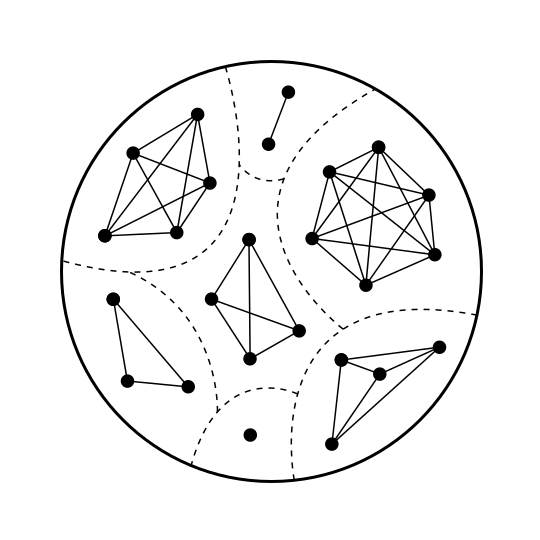
\includegraphics[scale=0.5]{equiv}
\end{figure}
\pagebreak 
~ 

\begin{tikzpicture}[remember picture, overlay, start chain, node distance=-2mm, shift={(-18mm, -12mm)}]
    \node [on chain]  {\pgfornament[width=1.72cm, color=darkscarlet]{158}};
\end{tikzpicture}
\subsection{Partitions and equivalence}

\lettrine{A}{  partition } $\mathcal{P}$ of a set $A$ is a set s.t. every $P \in \mathcal{P}$
is a subset of $A$, $P_1 \cap P_2 = \emptyset$ for any $P_1, P_2 \in
\mathcal{P}, P_1 \neq P_2$; and $\bigcup_{P \in \mathcal{P}} P = A$.

Given a partition $\mathcal{P}$ of a set $A$, a valid binary relation is 

\begin{align*}
    R_{\mathcal{P}} = \left\{ (a, b) : a, b \in  S \text{ for some } S \in
    \mathcal{P} \right\} 
\end{align*}

Observe that $R_{\mathcal{P}}$ is an equivalence relation. First of all,
$aR_{\mathcal{P}}a$ because $a$ is always in the same partition than $a$.
Furthermore, if $aR_{\mathcal{P}}b$ and $bR_{\mathcal{P}}c$ then $a$ and $c$ are
in the same partition. Lastly, if $a$ is in the same partition than $b$, then
$b$ is in the same partition than $a$ (symmetry).

Furthermore, if $R ~ \ddot{\propto} ~A$ is an arbitrary equivalence relation, then $A
/ R$ is a partition of $A$. To each element $a \in A$ corresponds some $a / R$
that contains \textit{at least} $a$; from this follows trivially that
$\bigcup_{a \in A} a / R = A$. Furthermore, if $a / R \neq b / R$ for some $a, b
\in  A$, then $a / R \cap b / R = \emptyset$---otherwise, some element $c \in A$
equivalent to $a$ and $b$ should exist, but this would contradict the hypothesis
that $a$ and $b$ are not equivalent. That $a / R \subseteq A$ for every $a \in
A$ follows trivially from the definition of equivalence class.

\begin{theorem}
    Let $A$ an arbitrary set, $\mathscr{P}_A$ the set of all partitions of $A$
    and $\mathscr{R}_A$ the set of all binary equivalence relations over $A$.
    Then 

    \begin{align*}
        \mathscr{P}_A &\mapsto \mathscr{R}_A &\mathscr{R}_A  &\mapsto \mathscr{P}_A \\ 
        \mathcal{P} &\mapsto R_{\mathcal{P}} & R &\mapsto A / R
    \end{align*}


    are bijections one the inverse of the other.
\end{theorem}


\small
\begin{quote}

\begin{pro}
    Complete.
\end{pro}

\end{quote}
\normalsize


\small
\begin{quote}

\begin{problem}
    Say true, false or imprecise the following statements.
\end{problem}

\textit{(1)} If $\mathcal{P}$ a partition of $X$ and $x \in X$, then $x /
\mathcal{P} \in \mathcal{P}$.

\begin{quote}
    Imprecise. $\mathcal{P}$ is a partition, not a binary relation, and thus the
    expression $x / \mathcal{P}$ is undefined.
\end{quote}

\textit{(2)} $\mathcal{P} = \left\{ 1, 3 / 2, 4 / 5, 6 \right\} $ is a partition
of $\left\{ 1, 2, 3, 4, 5, 6 \right\} $.

\begin{quote}
    Imprecise. The expression $3 / 2, 4 / 5$, etc. are undefined.
\end{quote}

\textit{(3)} If $\mathcal{P}$ a partition of $X$, then $\mathcal{P} \cap X =
\emptyset$.

\begin{quote}
    The statement is true. The set $\mathcal{P}$ contains \textit{sets} of
    elements of $X$; the set $X$ contains elements of $X$. Therefore, each $P
    \in \mathcal{P}$ is of a different type than each $x \in X$.
\end{quote}

\textit{(4)} If $R ~ \ddot{\propto} ~ A$, then $A \cap A / R = \emptyset$.

\begin{quote}
    We know $A / R$ is a partition of $A$, and in the previous problem we have
    already stated that $A \cap \mathcal{P} = \emptyset$ for any partition
    $\mathcal{P}$ of $A$. So the statement is true.
\end{quote}

\textit{(5)} If $R ~ \ddot{\propto} ~ A$ and there is a bijection between $A$
and $A / R$, then $R = \left\{ (x, y ) \in A^2  : x = y \right\} $.

\begin{quote}
    The statement is false. Consider $A = \mathbb{N}$ and $R$ the equivalence
    relation s.t. $A / R$ is the partition 
    
    $$\left\{ \left\{ 1 \right\}, \left\{
    2, 3\right\}, \left\{ 4, 5, 6 \right\}, \left\{ 7, 8, 9, 10 \right\}, \ldots
\right\} $$

    Then $F(1) = \left\{ 1 \right\} , F(2) = \left\{ 2, 3 \right\}, F(3) =
    \left\{ 4, 5, 6 \right\}, \ldots  $ is a bijection.

    It is interesting to study the finite case, however. If $A = \left\{ a_1,
    \ldots, a_n \right\} $ a finite set,and $F$ is bijective, we must have

    \begin{align*}
        F(a_1) = X_1, \ldots, F(a_{n}) = X_{n}
    \end{align*}

    with $X_i \neq X_j$ for $i, j \in [1, n]$. In other words, $|A / R| = |A|$, which implies $A / R$
    is a partition of $A$ into singleton sets. And because every element must be
    equivalent to itself, $A / R = \left\{ \left\{ a_1 \right\}, \ldots, \left\{
    a_n\right\}   \right\} \Rightarrow R = \left\{ (x, y) \in A^2 : x = y
    \right\} $.


\end{quote}

\end{quote}
\normalsize
\pagebreak

\begin{tikzpicture}[remember picture, overlay, start chain, node distance=-2mm, shift={(-18mm, -12mm)}]
    \node [on chain]  {\pgfornament[width=1.72cm, color=darkscarlet]{158}};
\end{tikzpicture}
\subsection{Functions with domain $A / R$}

\lettrine{H}{aving} defined a space of equivalence class $A / R$, it is natural 
to study functions over this space. In general, functions of the form $f : A /
R \mapsto B$ are ambiguous. For example, if we define $f(a / R) = f([a]) = a^2$
and $R$ is the relationship "has the same parity", then the fact that $[2] =
[4]$ would lead us to expect $f([2]) = 4 = f([4]) = 16$.

Notwithstanding, one of the fundamental ideas of modern algebra relates to a
function of precisely this form:

\begin{theorem}
    If $f : A \mapsto B$ is onto, then $\overline{f}(a / ker ~ f) = f(a)$
    defines a bijection $\overline{f} : A / ker ~ f \mapsto B$.
\end{theorem}


\small
\begin{quote}

\begin{pro}
    
\textit{(Is a function)} Observe that $\overline{f}(a / ker ~ f) = f(a)$
is uniquely determined for any $a \in A$.

\textit{(Injective)} Let $a_1, a_2 \in A$ arbitrary elements
with $a_1 / ker ~ f \neq a_2 / ker ~ f$. Assume $\overline{f}(a_1) =
\overline{f}(a_2)$. Then $f(a_1) = f(a_2)$, which entails $(a_1, a_2) \in ker ~
f$, which contradicts the assumption. Then $\overline{f}$ is injective.

\textit{(Surjective)} Let $b \in B$ an arbitrary element. Since $f$ is
surjective, $b = f(a)$ for some $a \in A$. From this follows $b = \overline{f}(a
/ ker ~ f)$. 

Since $\overline{f}$ is injective and surjective, $\overline{f}$ is a bijection.
\end{pro} 

\end{quote}
\normalsize

The theorem above guarantees, for any surjective $f$, the existence of a mapping from the quotient space
$A / ker ~ f$ onto $I_f$.


\small
\begin{quote}

\begin{problem}
    Say true, false or imprecise for the following statements.
\end{problem}

\textit{(1)} Let $R = \left\{ (x, y) \in \mathbb{Z}^2 : 2 \mid x - y \right\} $.
The equation $f(n / R) = \frac{1}{n^2 + 1}$ correctly defines a function.

\begin{quote}
    False. Observe that 

    $$\mathbb{Z} / R =  \left\{ \left\{ z \in \mathbb{Z} : z
    \text{ is even }\right\}, \left\{ z \in \mathbb{Z} : z \text{ is odd }
\right\}   \right\} $$

We would then expect $f(0 / R) = f(2 / R) \iff 1 = \frac{1}{5}$. ($\bot$)

\end{quote}

\textit{(2)} If $R ~ \ddot{\propto} ~A$ then $f : A / R \mapsto A$ defined as
$f(a / R) = a$ is onto.

\begin{quote}
    Imprecise because $f$ is not necessarily a function and hence we cannot say
    it is onto.
\end{quote}


\end{quote}
\normalsize


\pagebreak
\begin{tikzpicture}[remember picture, overlay, start chain, node distance=-2mm, shift={(0mm, 10mm)}]
    \foreach \i in {1,...,3}
    \node [on chain]  {\pgfornament[width=6.42cm, color=darkscarlet]{71}};
\end{tikzpicture}
\section{Partial orders}

\begin{definition}
    If $R \propto A$ is reflexive, transitive and anti-symmetric, then it is a
    partial order.
\end{definition}

We use $\leq$ to denote the binary relation that is a partial order. Because we
define $\leq$ as a binary relation, we must emphasize that $\leq$ denotes a set
of 2-uples. Furthermore, $<$ denotes $\left\{ (a, b) \in ~ \leq ~ : a \leq b \land a
\neq b\right\} $. 

\begin{definition}
    Let $\leq$ be a partial order over $A$. If $a < b$ and there is no $z$ s.t.
    $a < z$ and $z < b$, then we write $a \prec b$ and read "$b$ covers $a$" or
    "$a$ is covered by $b$".
\end{definition}

Observe that $\prec$ is itself the binary relation 
$$\left\{ (a, b) \in A^2 : a <
b \land \neg \left( \exists z \in A : a < z \land z < b \right) \right\} $$

\begin{definition}
    We say $\leq$ is a total order over $A$ if it is a partial order s.t. $x
    \leq y$ or $y \leq x$ for any $x, y \in A$.
\end{definition}

Partially or totally ordered sets are pairs $(P, \leq)$ where $\leq$ is a
partial or total order (respectively) over $P$.

\begin{tikzpicture}[remember picture, overlay, start chain, node distance=-2mm, shift={(-18mm, -12mm)}]
    \node [on chain]  {\pgfornament[width=1.72cm, color=darkscarlet]{158}};
\end{tikzpicture}
\subsection{Maximum, minimum, maximal, minimal}

Given a poset $(P, \leq)$, $x$ is a maximum if $a \leq x$ for all $a \in P$. The
definition of a minimum is analogous.  

\begin{theorem}
    If $(P, \leq)$ a poset, then $(P, \leq) $ has at most one maximum.
\end{theorem}


\small
\begin{quote}

    \begin{pro}
         Assume $(P, \leq) $ is a poset with two distinct maximums $x, y$. By
         definition then $x \leq y$ and $y \leq x$. By anti-symmetry we have $x
         = y$, which is a contradiction.
    \end{pro}

\end{quote}
\normalsize

Given a poset $(P, \leq) $, we use $1$ to denote its maximum and $0$ to denote
its minimum, if they exist. 

~ 

A maximal element of a poset $(P, \leq) $ is any $a \in P$ s.t. there is no $b
\in P$ s.t. $a < b$. In other words, a maximal element is an element that has no
successor in the order. Similarly, $a \in P$ is minimal if there is no $b \in P$
s.t. $b < a$. In other words, a minimal element is one that has no predecessor.


\small
\begin{quote}

\begin{problem}
    True or false: If $(P, \leq) $ a poset and $a \in P$ is not a maximum, then
    $a < b$ for some $p \in B$.
\end{problem}

False. Consider any poset $(P, \leq) $ that has $n > 1$ maximals $m_1, \ldots,
m_n$.
Then, for any $i, j = 1, \ldots, n$, $m_i$ is not a maximum (because $m_j \not<
m_i$) but $m_i \not< b$ for all $b \in B$. For an example of a poset with $n =
3$ maximals, see the graph below.

\begin{center}
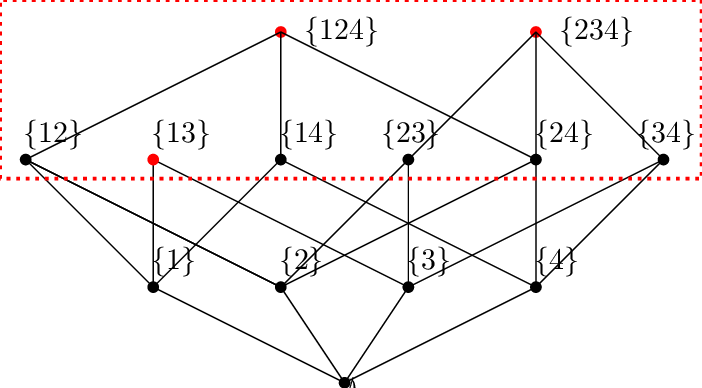
\includegraphics[scale=1]{threemaximals}
\end{center}

\begin{problem}
    True or false: If $(P, \leq) $ a poset without maximal elements, then $P$ is
    infinite.
\end{problem}

False, but only for a special case. If $P \neq \emptyset$, then it is true that
for any $a_1 \in P$ there is some $a_2$ s.t. $a_1 < a_2$, and this extends to
infinity: $a_1 < a_2 < \ldots $. However, if $P = \emptyset$, then the only
binary relation over $\emptyset$ is $\emptyset^2 = \emptyset$, which gives the
poset $(\emptyset, \emptyset)$. This poset is not only a partial order but a
total order; it contains no maximal elements, and yet it is not infinite.

\end{quote}
\normalsize


\begin{tikzpicture}[remember picture, overlay, start chain, node distance=-2mm, shift={(-18mm, -12mm)}]
    \node [on chain]  {\pgfornament[width=1.72cm, color=darkscarlet]{158}};
\end{tikzpicture}
\subsection{Supremum and infimum}
Let $(P, \leq) $ a poset and $S \subseteq P$. We say $a \in P$ is an upper bound
of $S$ in $(P, \leq) $ when $b \leq a$ for all $b \in S$. 

\begin{quote}
    \textbf{Note}. $\emptyset \subseteq P$, so what's the deal? Well, every
    element in $\emptyset$ (which is no element at all) is lesser than any $a
    \in P$. In other words, every element in $P$ is an upper bound of
    $\emptyset$.

    \textbf{Note 2.} For any given $S \subseteq P$, many upper bounds may exist
    (see the previous note).
\end{quote}

An element $a \in P$ is called the \textit{supremum} of $S$ in $(P, \leq) $ when
two properties hold: 

\begin{quote}
\begin{itemize}
    \item $a$ is an upper bound of $S$ in $(P, \leq) $ 
    \item For any $b \in P$, if $b$ is an upper bound of $S$ in $(P, \leq) $,
        then $a \leq b$.
\end{itemize}
\end{quote}

In other words, $a$ is a supremum if it is the lesser upper bound. It is always
unique.


\small
\begin{quote}

    \textbf{Example.} Let $(\mathbb{N}, \leq)$ denote the usual order over
    $\mathbb{N}$ and $S = \left\{ 1, 2, 3 \right\} $. Any natural $n \geq 3$ is an upper
    bound of $S$ in $(\mathbb{N}, \leq)$. However, $3$ is the only supremum of
    $S$.

\end{quote}
\normalsize

The definitions of the lower bound and the infimum are analogous. A lower bound
of $S \subseteq P$ in $(P, \leq) $ is any $a \in P$ s.t. $a \leq b$ for all $b
\in S$. The infimum is the greatest lower bound, or the lower bound $a$
satisfying that any lower bound $a'$ is s.t. $a' \leq a$.


\small
\begin{quote}

\begin{problem}
    Prove that if $a, a'$ are supremums of $S$ in $(P, \leq) $, then $a = a'$.
\end{problem}

By definition, $a, a'$ are the least upper bounds of $S$. If $a < a'$ then $a'$
is no longer the least upper bound and hence $a' \leq a$. The same reasoning
gives $a \leq a'$. Then, by anti-symmetry, $a = a'$.

\end{quote}
\normalsize

The previous problem shows that we can speak of \textit{the} supremum of $S
\subseteq P$ for any poset $(P, \leq) $.


\small
\begin{quote}

\begin{problem}
    Let $(P, \leq) $ a poset. 

    \textit{(1)} If $a \leq b$ then $\text{sup}\{a, b\}
    = b$. 

    \textit{(2)} Find $\left\{ a \in P : a \text{ is upper bound of }
    \emptyset \text{ in } (P, \leq)  \right\} $. 

    \textit{(3)} If the supremum of
    $\emptyset$ in $(P, \leq) $ exists, it is a minimum element of $(P, \leq) $.
\end{problem}

\textit{(1)} The statement is trivially true. 

\textit{(2)} Assume $P \neq \emptyset$. Since $\emptyset \subseteq P$ it is
correct to speak of the upper bound of $\emptyset$ in $(P, \leq) $. However, any
element $a \in P$ is an upper bound of $\emptyset$ in $(P, \leq) $. The reason
is that to prove $a \in P$ is \textit{not} an upper bound of $\emptyset$, we
should find some $x \in \emptyset$ s.t. $x \not\leq a$---in other words, because
the definition of upper bound involves a universal quantifier, its negation
involves an existential, a counter-example. And since $\emptyset$ has no
elements, there is no such counter-example. In conclusion, 

\begin{align*} \left\{ a \in  P : a \text{ is upper bound of } \emptyset \text{
in } (P, \leq)  \right\} = P \end{align*}

However, if $P = \emptyset$ (and therefore $\leq ~= \emptyset = \emptyset^2$), there is no
upper bound of $\emptyset$ in $(\emptyset, \emptyset)$.

\textit{(3)}  Due to \textit{(2)}, if the supremum exists then $P \neq \emptyset$.
Then any $a \in P$ is an upper-bound of $\emptyset$,
and the supremum is some $m \in P$ s.t. $m \leq a$ for any $a \in P$. 
$\therefore $ The supremum is the minimum of $(P, \leq)$.

\begin{problem}
    Give a finite poset with three elements $x_1, x_2, x_3$ s.t. \textit{(1)}
    $\left\{ x_1, x_2, x_3 \right\} $ is an anti-chain, meaning that $x_i
    \not\leq x_j$ when $i \neq j$; \textit{(2)} $\text{sup}\{x_i, x_j\} $
    doesn't exist for any $i \neq j$; \textit{(3)} $\text{sup}\{x_1, x_2,x_3\} $
    exists.
\end{problem}

A poset that satisfies this can be any that has the following Hasse diagram:

\begin{center}
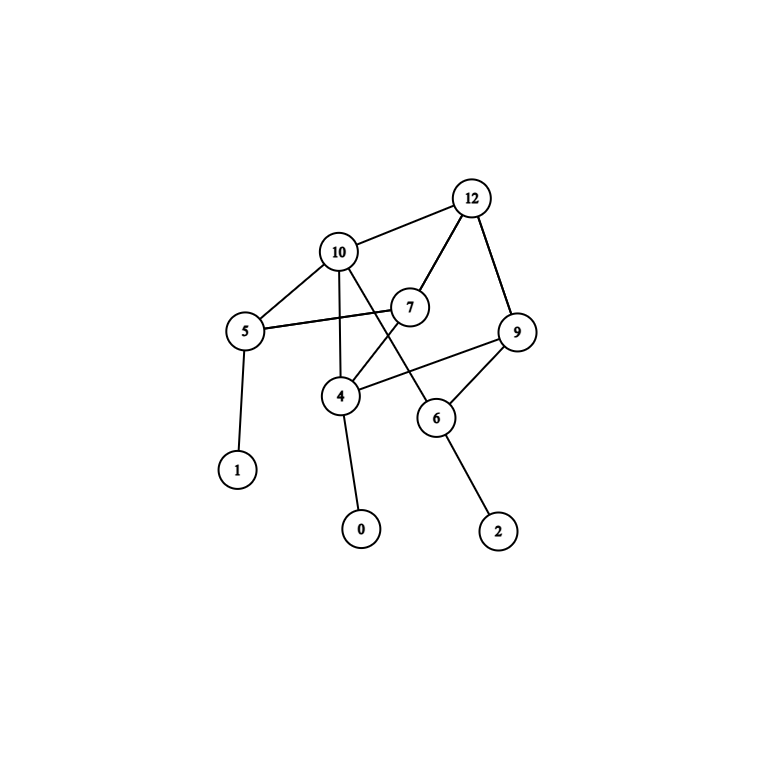
\includegraphics[scale=0.3]{graph}
\end{center}

Here, $0, 1, 2$ are $x_1, x_2, x_3$. The supremum on any pair of them does not
exist because each $\left\{ x_i, x_j \right\} $ has two upper bounds that are
not ordered with respect to one another. For example, the two smallest upper
bounds of $\left\{ 1, 0 \right\} $ are $10, 7$. But $10 \not\leq 7$ and $7
\not\leq 10$. However, $\text{sup}\{0, 1, 2\} = 12 $.

\begin{problem}
    If $(P, \leq) $ a poset and $a = \text{sup}(S)$ then $a = \text{sup}(S \cup
    \left\{ a \right\} )$.
\end{problem}

The statement is true. Our hypothesis is that $x \leq a$ for any $x \in S$, and $a
\leq b$ for any upper-bound $b$ of $S$. This evidently still holds for $S \cup
\left\{ a \right\} $, because $a \leq a$.

\begin{problem}
    Let $(P, \leq) $ a poset and $a \in P$. Then $a$ is a maximum of $(P, \leq)
    $ iff $a = \text{sup}(P) $.
\end{problem}

($\Rightarrow$) Assume $a$ is a maximum of $(P, \leq) $. Then $x \leq a$ for all
$x \in P$. Then $a$ is an upper-bound of $P$. Furthermore, if there were some $u
\in P$ s.t. $u$ is an upper bound and $u < a$, then by definition $u$ would not
be an upper-bound of $P$ because $a \not\leq u$. Then $a$ is the least upper
bound of $P$. $\blacksquare$

($\Leftarrow$) Assume $a$ is the supremum of $P$. Then $x \leq a$ for all $x \in
P$. The definition of a supremum of $S \subseteq P$ over $(P, \leq) $ requires
that the supremum be an element of $P$. Then $a \in P$. Then by definition $a$
is the maximum of $P$.

\textbf{Note.} The problem reveals a property; namely, that if $S \subseteq P$
and $\text{sup}(S)$ over $(P, \leq) $ satisfies $\text{sup}(S) \in S$, then this
supremum is the maximum of $(S, \leq)$. Alternatively, this can be stated as
follows: \textit{The maximum of a poset $(P, \leq) $, if it exists, is the
supremum $m$ of $P$ over $(P, \leq) $ whenever $m \in P$ }.

\begin{problem}
    Give true, false or imprecise.
\end{problem}

\textit{(1)} If $(P, \leq) $ a poset and $S \subseteq P$, then $a =
\text{sup}(S)$ in $(P, \leq) $ iff $a \in S$ and $b \leq a$, for all $b \in  S$.

\begin{quote}
    False. It is not necessary that $\text{sup}(S) \in S$. Consider the last
    graph we gave, where $\text{sup}\left\{ 0, 1, 2 \right\} = 12 $ is not in $\left\{
    0, 1, 2 \right\} $.
\end{quote}

\textit{(2)} Let $(P, \leq) $ a poset and $S \subseteq P$ and $a \in P$ an upper
bound of $S$. If $a$ is not the supremum of $S$, then there is some upper bound
$b$ of $S$ s.t. $b < a$.

\begin{quote}
    The statement is false. If $a$ is an upper bound of $S$ but it is not the supremum,
    it could very well be the case that another upper bound $b$ exists, with $a
    \not < b$ and $a \not > b$. 

    For an example, go at the last graph we showed;
    imagine the maximum (i.e. $12$) does not exist. Then consider that $10$ is
    an upper bound of $\left\{ 0, 1 \right\} $ but not a supremum, and yet there
    is no upper bound $b$ of $\left\{ 0, 1 \right\} $ s.t. $10 < b$.
\end{quote}

    \begin{problem}
        Let $P = \left\{ 0 \right\} \cup \left\{ x \in \mathbb{R} : 1 < x \leq 2
        \right\} $. Let 

        $$\leq = \left\{ (x, y) \in P^2 : x \leq y \right\} $$

        Let $S = \left\{ x \in \mathbb{Q} : 1 < x \leq 2 \right\} $. Does $S$
        have an infimum over $(P, \leq) $?
    \end{problem}


\small
\begin{quote}


    The order is the usual order, but over $P = \left\{ 0 \right\}  \cup (1, 2]$.
    The set $S$ (and in fact $P$ as well) has only one lower bound over $(P,
    \leq) $; namely, $0$. Observe that $1$ is not a lower bound because $1
    \not\in P$, and there is no such thing as the "first rational number". Since
    $0$ is the \textit{only} lower bound it is also the greatest lower bound.

\end{quote}
\normalsize


    \begin{problem}
        Say true or false. Let 

        $$\mathcal{D} \left( (x_0, y_0), r \right) = \left\{ (x, y) \in
        \mathbb{R}^2 : (x - x_0)^2 + (y - y_0)^2 \leq r^2 \right\} $$

        Let $P = \left\{ \emptyset \right\} \cup \left\{ \mathcal{D}\left( (x_0,
        y_0), r \right) : x_0, y_0 \in \mathbb{R}, r > 0  \right\} $. In the
        poset $(P, \subseteq ) $, there is always $\text{inf}\left\{ D_1, D_2
        \right\} $, for any $D_1, D_2 \in P$.
    \end{problem}


\small
\begin{quote}

     $\mathcal{D}\left( (x_0, y_0), r \right) $ is the set of
     points within a circumference with center $(x_0, y_0)$ and radius $r$. So
     $P$ is the set of all disks, including $\emptyset$. Two disks may be
     related in one and only one of the ways schematized by the following Venn diagrams:

     \begin{center}
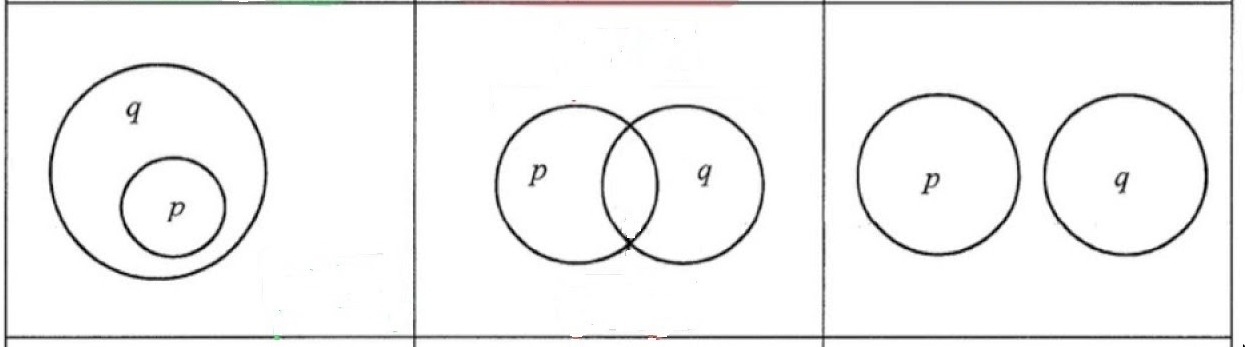
\includegraphics[scale=0.2]{circles}
\end{center}

Formally, for $D_1, D_2 \in P$, the image depicts the following exhaustive and
mutually exclusive cases: 

\begin{itemize}
    \item $D_1 \subseteq  D_2$, 
    \item $ D_1 \cap D_2 \neq \emptyset$ but $D_1 \not\subseteq D_2$
    \item $D_1 \cap D_2 = \emptyset$. 
\end{itemize}

It is easy to prove that in the first and third cases, there is an infimum.
However, consider the case $D_1 \cap D_2 \neq \emptyset$ with $D_1 \not\subseteq
D_2$. Let $D_3$ a disk s.t. $D_3 \subseteq D_1 \cap D_2$---this is, $D_3$ is an
arbitrary, non-empty lower bound of $\left\{ D_1, D_2 \right\} $. Then, given
any arbitrary $(z_1, z_2) \not\in D_3$ that
lies in $D_1 \cap D_2$, we can define $D_z = \mathcal{D}((z_1, z_2), \epsilon)$, with
$\epsilon > 0$ a quantity sufficiently small to guarantee $D_z \cap D_3 =
\emptyset$ and $D_z \in D_1 \cap D_2$. It is evident that $D_z$ is a lower bound
of $\left\{ D_1, D_2 \right\} $; but since $D_z \not\subseteq D_3$ we cannot say
$D_3$ is the greatest lower bound.

The argument above holds for any lower bound $D_3 \subseteq D_1 \cap D_2$. In
general terms, we have shown that, in the case $D_1 \cap D_2 \neq \emptyset, D_1
\not\subseteq D_2$, for any lower bound $D_3$ of $\left\{ D_1, D_2 \right\} $,
we can find a lower bound $D_z$ that is not a subset of $D_3$. Therefore no
greater lower bound exists and there is no infimum. Thus, the statement is
false.

\end{quote}
\normalsize



\begin{tikzpicture}[remember picture, overlay, start chain, node distance=-2mm, shift={(-18mm, -12mm)}]
    \node [on chain]  {\pgfornament[width=1.72cm, color=darkscarlet]{158}};
\end{tikzpicture}
\subsection{Poset homomorphism}

Let $(P, \leq), (Q, \leq')  $ two posets. A function $F : P \mapsto Q$ is called
a homomorphism from $(P, \leq) $ to $(Q, \leq')$ iff 

\begin{align*}
    \forall x, y \in P : x \leq y \Rightarrow F(x) \leq' F(y)
\end{align*}


We say $F$ is an isomorphism of $(P, \leq) $ in $(Q, \leq') $ if $F$ is a
bijective homomorphism and $F^{-1}$ is a homomorphism from $(Q, \leq') $ in
$(P, \leq) $. 


\small
\begin{quote}

\textbf{Note.} Not all bijective homomorphism satisfy the last property. For
example, 

\begin{align*}
    P &= \left( \left\{ 1, 2 \right\}, \left\{ (1, 1), (2, 2) \right\}\right) \\
    Q &= \left( \left\{ 1, 2 \right\}, \left\{ (1, 2),(2, 2), (1, 2)
\right\}   \right) 
\end{align*}

Then $F : \left\{ 1, 2 \right\} \mapsto \left\{ 1, 2
\right\} $ with $F(1) = 1, F(2) = 2$ is a bijective homomorphism. However,
$F^{-1}$ is not a homomorphism because $1 \leq' 2$ and $F^{-1}(1) = 1, F^{-1}(2)
= 2, 1 \not\leq 2$.

\end{quote}
\normalsize


The following theorem states that an isomorphism preserves all the properties of
interest.

\begin{theorem}
    Let $(P, \leq), (Q, \leq') $ two posets. Assume $F$ is an isomorphism from
    $(P, \leq) $ to $(Q, \leq') $. Then $x \leq y$ iff $F(x) \leq' F(y)$.
    Furthermore, if $x$ is a maximum, a minimum, a maximal or a minimal of $(P,
    \leq) $, then $F(x)$ is that same thing of $(Q, \leq') $. Moreover, for any
    $x, y, z \in P$, $z = \text{sup}\left\{ x, y \right\} $ if and only if $F(z)
    = \text{sup}\left\{ F(x), F(y) \right\} $, and the same applies to the
    infimum. Lastly, $x \prec y$ if and only if $F(x) \prec' F(y)$.
\end{theorem}


\small
\begin{quote}

\begin{pro}
    Complete.
\end{pro}

\end{quote}
\normalsize


\small
\begin{quote}

\begin{problem}
    Prove that if $(P, \leq) , (Q, \leq') $ posets with an isomorphism $F$, then
    for all $x, y \in P$ we have $x < y \iff F(x) <' F(y)$.
\end{problem}

($\Rightarrow$) Assume $x < y$. Then $F(x) \leq' F(y)$. Assume $F(x) = F(y)$.
Then $F^{-1}(F(x)) = F^{-1}(F(y))$, which contradicts the assumption. Then $F(x) <'
F(y)$.

$(\Leftarrow)$ Assume $F(x) <' F(y)$. Then we have $x \leq y$ (because $F^{-1}$
is an homomorphism). If $x = y$ and $F(x) <' F(y)$, we have $F(y)$ covers $F(x)$
but $y$ does not cover $x$ ($\bot$). Then $x < y$.

\begin{problem}
    Now prove $x$ is a maximum iff $F(x)$ is a maximum.
\end{problem}

$(\Rightarrow)$ Assume $x \in P$ is a maximum of $(P, \leq) $. Then $\forall y
\in P : y \leq x$. Then $\forall y \in P: F(y) \leq' F(x)$. Then $F(x)$ is a
maximum of $(Q, \leq') $.

$(\Leftarrow)$ Assume $F(x)$ is a maximum of $(Q, \leq') $ with $x \in P$. Then
$\forall y \in P : F(y) \leq' F(x)$. Then $\forall y \in P : F^{-1} \left( F(y)
\right) \leq F^{-1} \left( F(x) \right) $ or rather $\forall y \in  P : y \leq
x$.

\begin{problem}
    Now prove $x \prec y \iff F(x) \prec F(y)$.
\end{problem}

Assume $x \prec y$ for $x, y \in P$. Then $y \leq x$ and for all $z \in P$ s.t.
$y \leq z$ we have $x \leq z$. The first fact gives $F(y) \leq' F(x)$. The
second fact gives $F(x) \leq F(z)$ for all $z \in P$ s.t. $y \leq z$. Then $F(x)
\prec' F(y)$ . The other side of the implication is left to the reader.

\begin{problem}
    Give true, false or imprecise for the following statements.
\end{problem}

\textit{(1)} If $(P, \leq) , (P, \leq') $ are finite and isomorphic, then $\leq
= \leq'$.

\begin{quote}
    True. Observe that $x \leq y \iff x \leq' y$ which by definition entails
    $(x, y) \in  \leq \iff (x, y) \in  \leq'$.
\end{quote}

\textit{(2)} If $(P, \leq) $ a poset s.t. every $F : P \mapsto P$ is
homomorphic from $(P, \leq) $ in $(P, \leq) $, then $|P| = 1$.

\begin{quote}

    False. Assume $P = \emptyset$. There is only one function $F : P \to P$,
    namely $\emptyset^2 = \emptyset$. This function is a homomorphism because no
    counter-example can be found to the defining properties of a homomorphism in
    the empty set. So $P = \emptyset$ satisfies the properties but $|P| \neq 1$.
\end{quote}

\end{quote}
\normalsize


\begin{tikzpicture}[remember picture, overlay, start chain, node distance=-2mm, shift={(-18mm, -12mm)}]
    \node [on chain]  {\pgfornament[width=1.72cm, color=darkscarlet]{158}};
\end{tikzpicture}
\subsection{Lattices}

A poset $(P, \leq) $ is called a lattice if for any $x, y \in P,
\text{sup}\left\{ x, y \right\} $ and $\text{inf}\left\{ x, y \right\} $ exist.
Informally, this means that any pair of elements in $P$ is related to some
common successor and some common predecessor in $P$. We use $(L, \leq)$ to
denote a lattice.


\small
\begin{quote}

\begin{problem}
    Prove that $(\mathbb{N}, \mid)$ is a lattice. Does it have maximum and
    minimum?
\end{problem}

We skip the proof that $(\mathbb{N}, \mid)$ is a poset. Let $n_1, n_2 \in \mathbb{N}$ two arbitrary numbers. Because the set
$\mathcal{D}(n_1, n_2) = \left\{ d \in \mathbb{N} : d \mid n_1, d \mid n_2
\right\} $ is a finite set over the natural numbers, it has a maximum. Of
course, from a lattice perspective, $\mathcal{D}(n_1, n_2)$ is the set of lower
bounds of $\left\{n_1, n_2 \right\} $. Then $\text{inf}\left\{ n_1, n_2 \right\}
=\max \mathcal{D}(n_1, n_2)$ is guaranteed to exist. The proof that
$\text{sup}\left\{ n_1, n_2 \right\} $ exists is similar.

Because $1 \mid n$ for any $n \in \mathbb{N}$, $1$ is a minimum. However, there
is no natural $m \in \mathbb{N}$ s.t. $n \mid m$ for every $n$, so the set lacks
a maximum.

\begin{problem}
    Show that if $(P, \leq)$ is a total order then it is lattice.
\end{problem}

   Assume $(P, \leq) $ is a total order. If $\ldots \leq p_0 \leq p_1\leq  p_2 < \ldots$ 
   is the (potentially infinite) order of $P$, then for any 
   $i, k \in \omega$,  $\text{sup}\left\{ p_i, p_{i + k} \right\} = p _{i + k}$
   and $\text{inf}\left\{ p_i, p_{i +k} \right\} = p_i$. Then $(P, \leq) $ is a
   lattice.  

   \begin{problem}
       If $(P, \leq) $ a lattice then $\text{sup}(S)$ exists for any $S
       \subseteq P$?
   \end{problem}

   The statement is false. $(\mathbb{N}, \leq)$ with $\leq$ the usual order is a
   total order and therefore a lattice, and $\text{sup}(\mathbb{N}) $ does not
   exist.

   \begin{problem}
       True or false: If $(P, \leq) $ a lattice and $S \subseteq P$, then $(S,
       \leq ~ \cap ~ S^2)$ is a lattice.
   \end{problem}

   False. Consider as a counter example $(\left\{ 1, 2, 3, 6 \right\}, \mid )$.
   It is evident that this is a lattice, and here 

   $$\mid ~ = \left\{ (1, 2), (1,3), (1,6), (2, 6), (3, 6)\right\} $$

   Now consider $\left( \left\{ 1, 2, 3 \right\}, \left\{ (1, 2), (1, 3)
   \right\}   \right) $. This is obviously not a lattice.

\begin{problem}
    True or false: If $(P, \leq) $ a lattice and $S \subseteq P$ non-empty and
    s.t. $(S, \leq ~ \cap S^2)$ a lattice, then for any $a, b \in S$,
    $\text{inf}\left\{ a, b \right\} $ in $(P, \leq) $ coincides with
    $\text{inf}\left\{ a, b \right\} $ in $(S, \leq ~ \cap S^2)$.
\end{problem}

Should be true. COMPLETE.

\begin{problem}
    Let $P \subseteq \mathcal{P}(\mathbb{N})$ and assume $(P, \leq)$ a lattice
    with 

    \begin{align*}
        \leq ~ = \left\{ (A, B) \in P \times P : A \subseteq B \right\} 
    \end{align*}

    Is $\text{inf}\left\{ A, B \right\} = A ~ \cap |_{P^2} B $?
\end{problem}

Since $(P, \leq) $ a lattice we know the infimum of any pair of elements always
exist. Let $A, B \in P$ and assume $\text{inf}\left\{ A, B \right\} = I $. Then,
by definition, $I \subseteq A$ and $I \subseteq B$. Furthermore, for any $I' \in
P$ s.t. $I' \subseteq A$ and $I' \subseteq B$ we have $I' \subseteq I$. It
follows that for every $x \in A \cap B$ we have $x \in I$. Then $I = A \cap B$.
And since we have imposed the condition $A, B \in P$, the restriction of the
intersection to $P^2$ satisfies what we have shown. The statement is true.

\begin{problem}
    If $(P, \leq) $ a lattice and $m$ is a maximal element of $(P, \leq) $,
    then $m$ is a maximum of $(P, \leq) $. Is this true if $(P, \leq) $ is not a
    lattice?
\end{problem}

The statement is true. Assume $m$ is not a maximum. Then either there is some
$m' \in P$ s.t. $m \leq m', m \neq m'$, or there is some $x \in P$
s.t. $x \not\leq m$. If the first case holds then $m$ is not maximal ($\bot$).
If the second case holds then $\text{sup}\left\{ x, m \right\} $ does not exist
and $(P, \leq) $ is not a lattice ($\bot$). Then $m$ is a maximum. $\blacksquare$


\end{quote}
\normalsize


\begin{tikzpicture}[remember picture, overlay, start chain, node distance=-2mm, shift={(-18mm, -12mm)}]
    \node [on chain]  {\pgfornament[width=1.72cm, color=darkscarlet]{158}};
\end{tikzpicture}
\subsection{Binary operations}

Given a set $A$, a binary operation over $A$ is a function $f : A^2 \to A$ s.t.
$\mathcal{D}_f = A^2$. A lattice has by definition two binary operations: inf and
sup. We will write $a \lor b$ and $a \land b$ to denote the supremum
and infimum of $\left\{ a, b \right\} \subseteq P$, respectively.

\textbf{Some properties with their proofs:} Assume $x, y \in (L, \leq)$ a
lattice.

\begin{quote}
    \textit{(1)} $x \leq x \lor  y$ 

    \begin{quote}
        \textbf{Proof.} $x \leq x \lor  y$ by definition of supremum, because $x
        \lor  y$ is the least $z \in L$ s.t. $x \leq z, y \leq z$.
    \end{quote}

    \textit{(2)} $x \land  y \leq x$
    \begin{quote}
        \textbf{Proof.} The proof is similar to the previous case.
    \end{quote}

    \textit{(3)} $x \lor  x = x$

    \begin{quote}
        \textbf{Proof.} $\text{sup}\left\{ x, x \right\} = \text{sup}\left\{ x
        \right\} $ and of course $x$ is the lesser element in $L$ s.t. $x \leq
        x$.
    \end{quote}

    \textit{(4)} $x \land  x = x$
    \begin{quote}
        \textbf{Proof.} Similar to the previous case.
    \end{quote}


    \textit{(5)} $x \lor y = y \lor  x$
    
    \begin{quote}
        \textbf{Proof.} Trivial; left to the reader.
    \end{quote}

    \textit{(6)} $x \land  y = y \land  x$


\end{quote}



\begin{theorem}
    Let $(L, \leq)$ a lattice. For any $x, y \in L$, we have $x \leq y \iff x
    \lor y = y$. Furthermore, $x \leq y \iff x \land y = x$.
\end{theorem}


\small
\begin{quote}

\begin{pro}
    Complete.
\end{pro}

\end{quote}
\normalsize


\begin{theorem}[Absortion laws]
    Let $(L, \leq)$ a lattice and $x, y, z \in L$. Then \textit{(1)} $x \lor (x
    \land y) = x$ and \textit{(2)} $x \land (x \lor y) = x$.
\end{theorem}


\small
\begin{quote}

\begin{pro}
    Complete.
\end{pro}

\end{quote}
\normalsize

\begin{theorem}[Order preservation]
    If $x \leq z$ and $y \leq w$, then $x \circ y \leq z \circ w$, with $\circ
    \in \left\{ \lor, \land \right\} $.
\end{theorem}

\small
\begin{quote}

\begin{pro}
    Complete.
\end{pro}

\end{quote}
\normalsize

\textbf{Some proving tips.}

\begin{itemize}
    \item If you want to prove $x \lor  y \leq z$, it suffices to show $x \leq
        z$ and $y \leq z$. 

        \begin{quote}
            \textit{Justification.} Assume $x \leq z, y \leq z$. Then $z$ is an
            upper bound of $\left\{ x, y \right\} $. Since $x \lor  y$ is the
            least upper bound, $x \lor y \leq z$.
        \end{quote}

    \item If you want to prove $z \leq x \land  y$, it suffices to show $z \leq
        x$ and $z \leq y$. 

        \begin{quote}
            \textit{Justification.} If $z \leq x, z \leq y$, then $z$ is a lower
            bound of $\left\{ x, y \right\} $. Then, because $x \land  y$ is the
            least lower bound of this set, $z \leq x \land  y$.
        \end{quote}
\end{itemize} 

\begin{theorem}[Associativity]
    For any $x, y, z \in L$ with $(L, \leq)$ a lattice, $(x \lor y) \lor z = x
    \lor (y \lor  z)$, and the same holds for $\land $.
\end{theorem}

\small
\begin{quote}

\begin{pro}
\textit{(1)} Firstly, we will prove $(x \lor  y) \lor  z \leq x
\lor  (y \lor  z)$. To do this, we will prove the expression to the right is an
upper-bound of the terms in the expressions to the left. 

\begin{quote}

    \textit{(1.1)} It follows directly from the definition of supremum that $x
    \leq x \lor  (y \lor  z)$. Furthermore, let $\varphi = y \lor  z$, so that
    by definition $y \leq \varphi$. Since $\varphi \leq x \lor  \varphi$ we have
    $y \leq x \lor \varphi$ by transitivity. In other words, $y \leq x \lor  (y
    \lor  z)$. Then $x \lor  (y \lor  z)$ is an upper bound of $\left\{ x, y
    \right\} $. Then $x \lor y \leq x \lor  (y \lor  z)$.

    \textit{(1. 2)} That $z \leq x \lor  (y \lor  z)$ is clear from the fact
    that $z \leq y \lor  z$ and $y \lor  z \leq x \lor  (y \lor  z)$ (apply
    transitivity).

\end{quote}

From \textit{(1.1, 1.2)} follows that $x \lor (y \lor  z)$ is an upper bound of
$\left\{ x \lor  y, z \right\} $. Then $(x \lor  y) \lor  z \leq x \lor  (y \lor
z)$. $\blacksquare$

\textit{(2)} In a similar way, we can prove that $x \lor  (y \lor  z) \leq (x
\lor  y) \lor  z$. Since $\varphi \leq \psi$ and $\psi \leq \varphi$ imply
$\varphi = \psi$ for any $\varphi, \psi \in L$, this concludes the proof.

\end{pro}

\end{quote}
\normalsize


\begin{theorem}
    If $(L, \leq)$ a lattice and $x, y, z \in L$, then $(x \land y) \lor (x
    \land z) = x \land (y \lor  z)$. 
\end{theorem}


\small
\begin{quote}

    \begin{pro}
        
\textit{(1)} Observe that $(x \land  y) \lor   (x \land  z) \leq
x$. The reason is that $x \land  y \leq x $ trivially, $x \land  z \leq x$
trivially, and therefore $x$ is an upper bound of $\left\{ x \land  y, x \land
z\right\} $. Then the supremum of this set is necessarily less than or equal to
$x$.

\textit{(2)} Observe that $(x \land  y) \lor  (x \land z) \leq y \lor  z$. The
reason is that $x \land  y \leq y \leq y \lor  z$ and $x \land  z \leq  
z \leq y \lor  z$. Then $y \lor  z$ is an upper bound of $\left\{ x \land  y, x
\land  z\right\} $, and then the supremum of this set is less than or equal to
$y \lor  z$.

\textit{(3)} Results \textit{(1)} and \textit{(2)} entail $(x \land  y) \lor (x
\land  z)$ is a lower bound of $\left\{ x, y \lor  z \right\} $. Then $(x \land
y) \lor  (x \land  z) \leq x \land  (y \lor  z)$.

Using the same tricks we can prove $x \land  (y \lor  z) \leq (x \land  y) \lor
(x \land  z)$, which completes the proof. $\blacksquare$
    \end{pro}

\end{quote}
\normalsize


\pagebreak
\begin{tikzpicture}[remember picture, overlay, start chain, node distance=-2mm, shift={(0mm, 10mm)}]
    \foreach \i in {1,...,3}
    \node [on chain]  {\pgfornament[width=6.42cm, color=darkscarlet]{71}};
\end{tikzpicture}
\section{Lattices as algebras}

We have treated lattices as a special kind of poset. However, a lattice can be
modeled as a special kind of algebra. In general, a lattice is any $3$-uple
$(L, \lor, \land)$ with $L$ a set and $\lor, \land$ binary relations over $L$
that satisfy the following properties: 


\small
\begin{quote}

    For any $x, y, z \in L$:

\begin{itemize}
    \item $x \lor x = x \land x$ 
    \item $x \lor y = y \lor x$ (Commutativity)
    \item $x \land y = y \land x$ (Commutativity)
    \item $(x \lor y) \lor z = x \lor (y \lor z)$ (Associativity)
    \item $(x \land y) \land z = x \land (y \land z)$ (Associativity)
    \item $x \lor (x \land y) = x $
    \item $x \land (x \lor y) = x$
\end{itemize}

\end{quote}
\normalsize

Viewed in this way, if $(L, \leq)$ a lattice \textit{in the poset} sense, then
we have $(L, \lor, \land)$ a lattice \textit{in the algebraice sense} where
$\lor, \land$ denote the supremum and infimum operators. More formally,

\begin{theorem}[Dedekind]
    If $(L, \lor, \land)$ a lattice, the binary relation $x \leq y \iff x
    \lor y = y$ is a partial order over $L$ and it satisfies $\text{sup}\left\{ x, y
    \right\} = x \lor y, \text{inf}\left\{ x, y \right\} = x \land y$, for any
    $x, y \in L$.
\end{theorem}


\small
\begin{quote}

\begin{pro}
    Complete.
\end{pro}

\end{quote}
\normalsize


\small
\begin{quote}

\textbf{Note.} The theorem above states that any lattice in the algebraic sense
\textit{induces} a lattice in the poset sense. The \textit{operations} which
define the algebra induce a partial order where these operations correspond to
the supremum and minimum.

\end{quote}
\normalsize


We call $\leq$ the partial order induced by $(L, \lor, \land)$ and $(L, \leq)$ the
poset induced by $(L, \lor, \land)$.

\begin{problem}
    Compute the cardinality of the set 

    \begin{equation*}
        S = \left\{ \left( \left\{ 1, 2,3 \right\}, \lor , \land   \right) : \left( \left\{ 1, 2, 3 \right\}, \lor , \land   \right)  \text{ is a lattice} \right\} 
    \end{equation*}
\end{problem}


\small
\begin{quote}

    The set consists of all possible lattices (in the algebraic sense) over
    $\left\{ 1, 2, 3 \right\} $, and thus we are interested in finding how many
    possible such lattices are there. Dedekind's theorem states that any such
    lattice induces a lattice partial order $\leq$ s.t. $(P, \leq)$ is a
    partial order and $a \leq b \iff a \lor b = b$. Thus, the question becomes
    how many lattice partial orders exist over $\left\{ 1, 2, 3 \right\} $.
    There are $3! = 6$ total orders that are evidently lattices. 
    
    The partial orders are of two kinds: no element is in relation to another,
    and one element is not in relation to the others. In the first case, the
    supremum between two elements does not exist and the poset is not a
    lattice. In the second case, the supremum between the isolated element 
    and any of the others does not exist.

    $\therefore $ There are $3! = 6$ lattices over a set of $3$ elements,
    and $|S| = 6$.
\end{quote}
\normalsize

\begin{problem}
    If $(L, \lor , \land )$ is a lattice then $(L, \land , \lor )$ is a lattice.
    What is the relation between the posets induced by them?
\end{problem}


\small
\begin{quote}

The lattice poset induced by the first lattice satisfies $x \leq y \iff x \lor
y = y$, while the one induced by the second lattice satisfies $x \leq y \iff x
\lor  y = x $. So the ordering between the two posets is inverse; i.e. if $a
\leq_1 b$ then $b \leq_2 a$. The Hasse diagrams of these posets will be
horizontal mirrors of each other. 

\end{quote}
\normalsize

\begin{problem}
    True, false or imprecise: If $(L, \lor , \land) $ a lattice and $t \in \lor$,
    then $Ti(t) = 3\text{-UPLE}$.
\end{problem}


\small
\begin{quote}

    $\lor $ is a function; i.e. a set of $2$-uples. So if $t \in \lor $
    we have $Ti(t) = 2$-uple. The statement is false.

\end{quote}
\normalsize


\begin{problem}
    True, false or imprecise: If $(L, \lor , \lor ) $ a lattice, 
    then $L$ has exactly one element.
\end{problem}


\small
\begin{quote}

    False. $(\emptyset, \lor , \lor)$ is a lattice for any function $\lor$, but
    $|\emptyset| \neq 1$. Only if we assume $L \neq \emptyset$ can we say the
    statement is true. And this because if more than one element existed, we
    would require that any pair $x \neq y$ in the induced lattice poset
    satisfies $\text{sup}\left\{ x, y \right\} = x \iff \text{inf}\left\{ x, y
    \right\} = y $. But if the functions inducing the supremum and infimum are the same, 
    this would entail $x \lor  y = x$ and $x \lor y = y$, which in turn implies
    $y \leq x$ and $x \leq y$. But then $\leq$ is not anti-symmetric, which 
    contradicts that $(L, \leq)$ is a lattice.

\end{quote}
\normalsize

\begin{problem}
    True, false or imprecise: If $(L, \lor , \land  ) $ a lattice, 
    then it is always the case that $\land  \leq \lor $.
\end{problem}


\small
\begin{quote}

    The statement is equivalent to $(\lor, \land ) \in \left\{ (x, y) : x \lor
    y = y \right\} \subseteq L^2 $. But clearly $\lor \not\in L, \land \not\in
    L$. The statement is false.

\end{quote}
\normalsize

\begin{problem}
    True, false or imprecise: If $(L, \lor , \land  ) $ a lattice, 
    then $\lor (x, y, z) = \land (x, y, z)$ for any $x, y, z \in L$.
\end{problem}


\small
\begin{quote}

    Imprecise. There are no $3$-argument functions $\lor ,\land $ defined 
    in this context.

\end{quote}
\normalsize

\pagebreak
\begin{tikzpicture}[remember picture, overlay, start chain, node distance=-2mm, shift={(-18mm, -12mm)}]
    \node [on chain]  {\pgfornament[width=1.72cm, color=darkscarlet]{158}};
\end{tikzpicture}
\subsection{Distributive lattice}

A lattice $(L, \lor, \land)$ is said to be distributive when, for any $x, y, z,
\in L$, we have $x \land (y \lor z) = (x \land y) \lor (x \land z)$. It can be
proven that if this property holds (distributivity of $\land$ over $\lor$), its
complementary property holds (distributivity of $\lor$ over $\land$). 

\begin{problem}
    Prove that $(\mathbb{R}, \max, \min)$ and $(\mathcal{P}(\mathbb{N}), \cup, \cap )$
    are distributive.
\end{problem}


\small
\begin{quote}

\textit{(1)} We skip the proof that $(\mathbb{R}, \max, \min)$ is a lattice.
Let $\land , \lor $ denote $\min$ and $\max$. Let $u = x \lor  y$ and $w = z
\land  u$. Let us examine the cases where $x \leq y$ and 
$y < x$, and let us use $A$ and $B$ to denote the expressions 
of the distributive property.

$( x \leq y )$ Here $A = x \land (y \lor  z) = x$, because 
$x \leq y \leq y \lor  z$. At the same time, 
$B =  x \lor (x \land  z) = x$ because $x \geq (x \land  z)$.
$\therefore A = B$. $\blacksquare$

$(y < x)$ Again, two cases. 

\begin{itemize}
    \item $(x \leq z)$ Here $y < x \leq z$. Then $A = x \land y = x$ 
and $B = y \lor x = x$. $\therefore A = B$. 
    \item $(z \leq x)$ Here $A = x \land (y\lor  z) = y \lor  z$. 
        Simultaneously, $B = y \lor z$.
        So $A = B$.
\end{itemize}


\textit{(2)} We will again inspect two cases given $A, B, C \in
\mathcal{P}(\mathbb{N})$. Observe that the order induced by these operations is
$\subseteq$, since $A \leq B \iff A \cup B = B$, and $A \leq B \iff A \cap B =
A$. We will use $\varphi, \psi$ to denote the sides of the distributive
property. 

$(A \subseteq B)$ Since $A \subseteq B \subseteq (B \cup C)$, we have 
$A \subseteq (B \cup C)$ and

\begin{align*}
    A &= A \cap (B \cup C) \\ 
      &= A
\end{align*}

Furthermore, $(A \cap B) \cup (A \cap C) = A \cup (A \cap C) = A$. Then $\varphi = \psi$. 

$(B \subseteq A)$ Similar to the previous excercise. COMPLETE.


\end{quote}
\normalsize


\begin{tikzpicture}[remember picture, overlay, start chain, node distance=-2mm, shift={(-18mm, -12mm)}]
    \node [on chain]  {\pgfornament[width=1.72cm, color=darkscarlet]{158}};
\end{tikzpicture}
\subsection{Sub-lattices and sub-universes}

If $(L, \land, \lor), (L', \land', \lor')$ are lattices, we say the first is a
sub-lattice of the other iff 

\begin{itemize}
    \item $L \subseteq L'$
    \item $\lor = \lor'\mid_{L \times L}$ and $\land = \land'\mid_{L \times L}$
\end{itemize}

We say $S \subseteq L$ is a sub-universe of $(L, \lor, \land)$ if $S \neq
\emptyset$ and $S$ is closed under $\lor, \land$.


\small
\begin{quote}

\textbf{Note.} The concepts of sub-lattice and sub-universe are similar but not
identical. A sub-universe of $(L, \lor, \land)$ is a \textit{set}; a sub-lattice
of $(L, \lor, \land)$ is a lattice. It is true that if $S$ is a sub-universe,
then $(S, \lor \mid_{S \times S}, \land \mid_{S \times S})$ is a sub-lattice,
and that every sub-lattice is obtained in this manner. In other words, there is
a bijection between sub-lattices and sub-universes. 


\end{quote}
\normalsize

\begin{problem}
    What are the sub-universes of:

    \textit{(1)} $\left( \mathcal{P}(\left\{ 1,2
    \right\}, \cup, \cap ) \right) $ 

    \textit{(2)} $\left( \left\{ 1, 2, 3, 6,
    12 \right\}, \gcd, \lcm  \right) $

    \textit{(3)} $\left( \mathbb{R}, \max, \min \right) $
\end{problem}


\small
\begin{quote}

    \textit{(1)} A sub-universe of a poset is a non-empty subset of the poset
    that is closed under $\land , \lor $. Since $\left\{ 1, 2 \right\} $ has
    two elements, no strict subset of it is a sub-universe. $\therefore $
    $\left\{ 1, 2 \right\} $ is the only sub-universe of $\left\{ 1, 2 \right\}
    $.

    \textit{(2)} The only subset which is not a sub-universe is $\left\{ 2, 3 \right\} $,
    (the primes) since $\gcd(2, 3) = 1$. Any other subset contains 
    either a prime in $\left\{ 2, 3 \right\} $ with non-prime numbers,
    or only non-prime numbers. It is easy to see that the subsets
    with non-prime numbers only,

    \begin{equation*}
        \left\{ 12, 6 \right\}, \left\{ 12, 6, 1 \right\}, \left\{ 1, 6 \right\}, \left\{ 1, 12 \right\} 
    \end{equation*}

    are closed under $\gcd$ and $\lcm$. The sets containing a prime among other
    elements are also cloesd. So the sub-universes of the set $S = \left\{ 1,
    2, 3,6,12 \right\} $ are $U = \left\{ W \in \mathcal{P}(S) : W \neq \left\{
    2,3 \right\} \land  |W| > 1  \right\} $.

    \textit{(3)} Every subset $S \subseteq \mathbb{R}$ with $|S| > 1$ is 
    closed under $\max$ and $\min$. Then the sub-universes of this 
    poset are all possible sets of real numbers with more than one 
    element.



\end{quote}
\normalsize


\begin{tikzpicture}[remember picture, overlay, start chain, node distance=-2mm, shift={(-18mm, -12mm)}]
    \node [on chain]  {\pgfornament[width=1.72cm, color=darkscarlet]{158}};
\end{tikzpicture}
\subsection{Lattice homomorphisms and isomorphisms}

Let $(L, \lor, \land), (L', \lor', \land')$ be lattices. A function $F : L
\mapsto L'$ is a lattice homomorphism from $(L, \lor, \land)$ in $(L', \lor',
\land')$ iff 

\begin{align*}
    F(x \circ y) = F(x) \circ' F(y)
\end{align*}

with $\circ$ either $\lor$ or $\land$. A homomorphism is called an isomorphism
when it is bijective and its inverse is a homomorphism as well. We write $(L,
\land, \lor)
\simeq (L', \land', \lor') $ to say that two lattices are isomorphic.

\begin{theorem}
    If $F$ is a bijective homomorphism between two lattices, then it is an
    isomorphism. 
\end{theorem}


\small
\begin{quote}

    \begin{pro}
 Assume $F$ a bijective homomorphism. Observe that, since 
$F$ is a homomorphism,

\begin{align*}
    F \left[F^{-1}(x) \circ F^{-1}(y)\right] &= F\left[ F^{-1}(x) \right] \circ' F \left[ F^{-1}(y) \right]  \\ 
                                             &=x \circ' y
\end{align*}

It follows that 

\begin{equation*}
    F^{-1}\left[ x \circ' y \right] &= F^{-1} \left[ F \left( F^{-1}(x) \circ F^{-1}(y) \right)  \right] \\ 
                                    &=F^{-1}(x) \circ F^{-1}(y)
\end{equation*}

$\blacksquare$
    \end{pro}

\end{quote}
\normalsize

\begin{theorem}
    Let $F$ an homomorphism from  $(L, \lor, \land) $ in $ (L', \lor',
    \land')$. Then $I_F$ is a sub-universe of $(L', \lor', \land')$, and in
    consequence $F$ is an homomorphism from $(L, \lor, \land)$ in $(I_F,
    \lor'\mid_{I_F \times I_F}, \land'\mid_{I_F \times I_F})$.
\end{theorem}


\small
\begin{quote}

\begin{pro}
    Complete
\end{pro}

\end{quote}
\normalsize


\begin{theorem}
    Let $(L, \lor, \land )$ and $(L', \lor ', \land ')$ lattices with associated
    posets $(L, \leq), (L', \leq')$. Then $F$ is an isomorphism of $(L, \lor ,
    \land )$ in $(L', \lor ', \land ')$ iff $F$ is an isomorphism from $(L,
    \leq)$ to $(L', \leq')$.
\end{theorem}

\small
\begin{quote}

\begin{pro}
    Complete
\end{pro}

\end{quote}
\normalsize


\begin{tikzpicture}[remember picture, overlay, start chain, node distance=-2mm, shift={(-18mm, -12mm)}]
    \node [on chain]  {\pgfornament[width=1.72cm, color=darkscarlet]{158}};
\end{tikzpicture}
\subsection{Lattice congruence}

A congruence over a lattice $(L, \lor , \land )$ is an equivalence relation
$\theta ~ \ddot{\propto} ~ L$ s.t. 

\begin{align*}
    x_1 \theta x_2 \text{ and } y_1 \theta y_2 \Rightarrow (x_1 \lor  y_1)
    \theta (x_2 \lor  y_2) \text{ and } (x_1 \land y_1) \theta (x_2 \theta y_2)
\end{align*}

This condition essentially requires that equivalence is preserved in the
lattice operations; i.e. the supremum/infimum between members of two classes
should be equivalent to the supremum/infimum between any other members of those
two classes. 

Because equivalence is preserved among the classes of equivalence in the
lattice operations, it is possible to define the supremum/infimum between 
two classes:

\begin{align*}
    x / \theta ~ \widetilde{\circ } ~ y / \theta = (x \circ y) / \theta
\end{align*}

with $\circ \in \left\{ \lor , \land  \right\} $.

\small
\begin{quote}

\textbf{Example.} \textit{(1)} Consider the lattice $\left( \left\{ 1, 2, 3, 4,
5, 6\right\}, \max, \min  \right) $. Let $\theta$ be the equivalence relation
induced by the partition $\left\{ \left\{ 1, 2 \right\}, \left\{ 3 \right\},
\left\{ 4, 5 \right\}   \right\} $. Then $\theta$ is a congruence. For example, 

\begin{align*}
    1\theta 2, 4 \theta 5 \text{ and } (1 \max 4) \theta (2 \max 5)
\end{align*}

The same can be verified for the $\min$ operation. Of course, we have that
$\left\{ 1, 2 \right\} \widetilde{\max} \left\{ 4, 5 \right\} = (1 \max  4) /
\theta = 4 / \theta = \left\{ 4, 5 \right\} $. 

\end{quote}
\normalsize

\begin{theorem}
    If $(L, \lor , \land )$ a lattice and $\theta$ a congruence relation of this
    lattice, then $(L / \theta, \widetilde{ \lor  }, \widetilde{ \land  }  )$ is
    a lattice.
\end{theorem}

We use $\widetilde{ \leq } $ to denote the partial order associated to the
lattice $(L / \theta, \widetilde{ \lor  }, \widetilde{ \land  }  )$.


\small
\begin{quote}
\begin{pro}
    
    Since $(L, \lor , \land )$ is a lattice, $x \lor   y = x \land  y $. By definition, 

    $$[x] \widetilde{ \lor  } [y] =  [ (x \lor y) ] = [(x \land  y)] = [x] \widetilde{ \land  } [y] $$

    Commutativity is similar (we give it only for $\widetilde{ \lor  } $):

    $$[x] \widetilde{ \lor  } [y] = [ (x \lor y) ] = [( y \lor  x )] = [y] \widetilde{ \lor  } [x]$$

    Associativity (we give it only for $\widetilde{ \lor  }  $):

    \begin{align*}
        ( [x] \widetilde{ \lor } [y] ) \widetilde{ \lor  } [z] &= \left[ \left( x \lor y \right)  \right] \widetilde{ \lor  } [z] \\ 
                                                               &= \left[ (x \lor y) \lor  z \right] \\ 
                                                               &=\left[ x \lor (y lor z) \right] \\ 
                                                               &= [x] \widetilde{ \lor  } \left( [y] \widetilde{ \lor  }  [z]\right) 
    \end{align*}

    Now we will prove $[x] \widetilde{ \lor  } ([x] \widetilde{ \land   } [y])
    = [x]$. But this can be done with words. The infimum $[x] \widetilde{ \land
    } [y] $ will be the equivalence class of the infimum between $x$ and $y$ in
    the original lattice. If the result is $[x]$ then the property follows
    immediately. If the result is $[y]$ we have $y \land  x = y \Rightarrow y
    \lor x = x$ which entails $[x] \widetilde{ \lor  }   [y] = [x]$. 

    Then $(L/\theta, \widetilde{ \land  }, \widetilde{  \lor   })$ is a
    lattice. $\blacksquare$


\end{pro}

\end{quote}
\normalsize


\begin{theorem}
    If $(L, \lor , \land )$ a lattice and $\theta$ a congruence over this
    lattice, then 

    \begin{align*}
        x / \theta ~ \widetilde{ \leq } y / \theta  ~ \iff y \theta (x \lor  y)
    \end{align*}

    for any $x, y \in L$.
\end{theorem}


\small
\begin{quote}

\begin{pro}
Recall that the order induced by a lattice $(L, \lor , \land )$
is $x \leq y \iff x \lor  y = y$. So to prove this theorem we must study
the order induced by $(L / \theta, \widetilde{ \land  }, \widetilde{  \lor   }
) $; namely, 

\begin{equation*}
    [x] \widetilde{ \leq }  [y] \iff [x] \widetilde{ \lor  } [y] = [y]
\end{equation*}

It is clear that if $[x] \widetilde{  \lor   } [y] = [y]$ we have $[(x \lor
y)] = [y]$, which is exactly the same as saying $(x\lor y)\theta y$. $\blacksquare$
\end{pro}

\end{quote}
\normalsize


\begin{theorem}
    If $F : (L, \land , \lor ) \mapsto (L', \land ', \lor ')$ an homomorphism,
    then $ker(F)$ is a congruence over $(L, \land , \lor )$.
\end{theorem}


\small
\begin{quote}
\begin{pro}
    
Let $\theta = ker(F)$ with $F$ a homomorphism between two
arbitrary lattices $(L, \land , \lor ), (L', \land ', \lor ')$. If $\theta =
\emptyset$ then $\theta$ is a congruence by lack of counter-examples. Assume
$\theta \neq \emptyset$.

Let $x_0, x_1, y_0, y_1$ be elements of $L$ s.t. $x_0 \theta x_1$ and $y_0
\theta y_1$. Then $F(x_0) = F(x_1)$ and $F(y_0) = F(y_1)$.
Since $x_0 \circ x_1 \in \left\{ x_0, x_1 \right\} $, we have 
$F(x_0 \circ x_1) = F(x_0)$, and $F(y_0 \circ y_1) = F(y_0)$.

We know $F(x_0 \circ y_0) \in \left\{ F(x_0), F(y_0) \right\} $, and $F(x_1
\circ y_1) \in \left\{ F(x_1), F(y_1) \right\} $. We wish to prove $F(x_0 \circ
y_0) \neq F(x_1 \circ y_1)$. The only problematic case is when the first
expression is $F(x_0)$ and the latter $F(y_1)$ or vice-versa.

Assume without loss of generality that $\circ = \lor$ and 

\begin{align*}
    \textit{(1)} ~ &F(x_0 \circ y_0) = F(x_0)\\
    \textit{(2)} ~ &F(x_1 \circ y_1) = F( y_1 )
\end{align*}

Prop. \textit{(1)} entails $(x_0 \lor y_0)\theta x_0$. Then, in the order
induced by $\theta$, $[y_0] \tilde{ \leq } [x_0]$. But $[y_0] = [y_1], [x_0] =
[x_1]$, and then $[y_1] \tilde{ \leq } [x_1]$. But then $(y_1 \lor x_1)\theta
x_1$. 

$\therefore $ $F(y_1 \lor  x_1) = F(x_1)$ and \textit{(2)} gives $F(x_1) = F(y_1)$.

$\therefore $ $F(x_0) = F(x_1) = F(y_1)$ and \textit{(1)} and \textit{(2)} give 
$F(x_0 \lor  y_0) = F(x_1 \lor  y_1)$. $\blacksquare$

\end{pro}

\end{quote}
\normalsize

\begin{theorem}
    Let $(L, \lor , \land )$ a lattice and $\theta$ a congruence over it. 
    Then $\pi_{\theta}$ is a homomorphism from $(L, \lor , \land )$ to 
    $(L / \theta, \widetilde{ \lor  }, \widetilde{ \land  } ) $, and 
    $\ker(\pi_{\theta}) = \theta$.
\end{theorem}


\small
\begin{quote}

    \begin{pro}
        
Let $x, y \in L$. Then 

\begin{equation*}
    \pi_{\theta}(x \circ  y) = (x \circ y) / \theta
                            = x / \theta ~ \widetilde{ \circ }  y / \theta\\ 
                            = \pi_{\theta}(x) ~ \widetilde{ \circ }  ~ \pi_{\theta}(y)
\end{equation*}

    Now, $\ker(\pi_\theta) = \left\{ (a, b) \in \mathcal{D}_{\pi_\theta}^2 :
        \pi_\theta(a)
    = \pi_\theta(b) \right\} $. Since $\pi_{\theta}$ is 
    a homomorphism, $\mathcal{D}_{\pi_\theta} = L$, and due 
    to the definition of canonic projection, 
    $\pi_\theta(x) = \pi_\theta(y) \iff x\theta y$.
    Then $\ker(\pi_\theta) = \left\{ (a, b) \in L : a\theta b \right\} $.
    This is trivially equal to $\theta$.
    \end{pro}


\end{quote}
\normalsize

\begin{problem}
    Give all the congruences of $(\left\{ 1, 2, 3, 6, 12 \right\}, \gcd, \lcm )$.
\end{problem}


\small
\begin{quote}


    Complete.


\end{quote}
\normalsize

\begin{problem}
    Let $\theta$ a congruence over $(L, \lor , \land )$. Prove 
    that, if $c \in L / \theta$,

    \textit{(1)} $c$ is a sub-universe of the lattice.

    \textit{(2)} $c$ is a convex subset of the lattice; i.e. for any 
    $x,y,z \in L$ 
    \begin{equation*}
        x,y \in c \text{ and } x \leq z \leq y \Rightarrow z\in c
    \end{equation*}
\end{problem}


\small
\begin{quote}

    \textit{(1)} A sub-universe is a non-empty subset of a lattice that 
    is closed under the lattice operations. That $c / \theta \subseteq L$ 
    is trivial, and it must be non-empty because each element is 
    at least equivalent to itself. Assume it is not closed under 
    the lattice operations; i.e. assume there are $x_0, x_1 \in c /\theta$
    s.t. $u = x_0 \circ x_1 \not\in c / \theta$. 

    Theorem \textbf{18} ensures that $\pi_{\theta}$ is a homomorphism from $(L,
    \lor , \land )$ to $(L / \theta, \widetilde{ \lor  }, \widetilde{ \land  }
    ) $. But by assumption:

    \begin{align*}
        \pi_{\theta}(x_0 \circ x_1) \neq c /\theta \Rightarrow \pi_{\theta}(x_0) ~\widetilde{ \circ } ~ \pi_{\theta}(x_1) \neq c / \theta
    \end{align*}

    But this entails $c / \theta ~ \widetilde{ \circ } ~ c / \theta \neq c / \theta$, 
    which is absurd because $(L / \theta, \widetilde{ \lor  }, \widetilde{
    \land  } ) $ is a lattice. Then $c / \theta$ must be closed and hence must
    be a sub-universe. $\blacksquare$

    \textit{(2)} Let $x, y, z \in L$. Assume $x, y \in c$ and $x \leq z \leq y$.
    We wish to prove this entails $z \in c$.

    Since $(L / \theta, \widetilde{ \land  }, \widetilde{ \lor  })  $ is 
    a lattice (\textbf{Theorem 15}), it induces a poset $(L, \widetilde{ \leq }) $
    s.t. 

    \begin{equation*}
        a \widetilde{ \leq } b \iff b\theta(a \widetilde{ \lor  } b)
    \end{equation*}

    Since $x \leq z \leq y$ we have 

    \begin{enumerate}
        \item $z \theta(x\lor z)$ 
        \item $y\theta(z \lor y)$
    \end{enumerate}

    In terms of the homomorphism $\pi_{\theta}$, this means 

    \begin{enumerate}
        \item $\pi_{\theta}(z) &= \pi_{\theta}(x) \widetilde{ \lor  } \pi_{\theta}(z)$
        \item $\pi_{\theta}(y) &= \pi_{\theta}(z) \widetilde{ \lor  } \pi_{\theta}(y)$
    \end{enumerate}

    Since $x, y \in c$ we have $\pi_{\theta}(x) = \pi_{\theta}(y)$. If we look
    at equations (1) and (2), this entails $\pi_{\theta}(z) = \pi_{\theta}(y)$.

    $\therefore  $ $z \in c$.
    
    
\end{quote}
\normalsize

\begin{problem}
    Say true, false or imprecise for the following statements, 
    where $(L, \lor , \land )$ is a lattice.
\end{problem}


\small
\begin{quote}

\textit{(1)} Let $S$ a sub-universe of the lattice and $\theta$ a congruence 
of $(S, \lor_{S\times S}, \land_{S\times S})$. There is a congruence 
$\lambda$ of $(L, \lor , \land )$ s.t. $\theta = \lambda \cap S^2$.

\textit{False}. See the \textit{Congruence extension property.}


\textit{(2)} Assume the lattice is distributive and $\theta$ is a congruence 
over it. Then $(L / \theta, \widetilde{ \lor  }, \widetilde{ \land  })$ is 
distributive.

The statement is true. Observe that for $x, y, z \in L$,

\begin{align*}
    x / \theta \widetilde{ \lor  } (y / \theta \widetilde{ \land  } z / \theta) &= x / \theta \widetilde{ \lor  } \left( \left( y \land  z \right) / \theta    \right)  \\ 
    &= \left( x \lor \left( y \land  z \right)  \right) /\theta \\ 
    &= \left( \left( x \lor  y \right) \land \left( x \lor  z \right)   \right) /\theta \\ 
    &=\left( x \lor  y \right) / \theta \widetilde{ \land  } \left( x \lor  z \right) / \theta \\ 
    &= \left( x /\theta \widetilde{ \lor  } y / \theta \right)  \widetilde{ \land  } \left( x / \theta  \widetilde{  \lor  } z / \theta\right) 
\end{align*}



\textit{(3)} Let $\theta$ a congruence over the lattice. If $u \in L$
is s.t. $u / \theta$ is a maximum of $(L, \lor , \land ) / \theta$,
then $u$ is a maximum of the original lattice.

The statement is imprecise. The symbol $(L, \lor , \land ) / \theta$
is undefined.


\end{quote}
\normalsize

\begin{problem}
    Let $(L, \lor , \land )$ a lattice, $\theta$ a congruence over it and 
    $\leq$ the order induced by $\lor $. Let $(L / \theta, \widetilde{\lor}, \widetilde{\land})$ the quotient lattice and $\widetilde{ \leq } $ the order induced by 
    $\widetilde{ \lor  } $. Prove that given $c_0, c_1 \in L / \theta$, 
    $c_0 \widetilde{ \leq }  c_1$ iff there are $x \in c_0, y \in c_1$ s.t. $x \leq y$.
\end{problem}


\small
\begin{quote}

$(\Rightarrow)$ Assume there are $c_0, c_1 \in L / \theta$ s.t. $c_0
\widetilde{ \leq } c_1 $. There must be elements $x, y$
s.t. $x / \theta = c_0$ and $y / \theta = c_1$.
By \textbf{Theorem 16} we have 

\begin{equation}
    y\theta(x \lor  y)
\end{equation}

If $x = y$ then $x \leq y$ and the result is trivial, so assume $x \neq y$.
Then $c_0 \neq c_1$.  If $x \lor  y = x$, equation (1) gives $y \theta x$,
which violates the fact that $c_0 \neq c_1$. So $x \lor  y = y$. 

$\therefore x \leq y$.

$(\Leftarrow)$ Assume there are $x \in c_0, y \in c_1 $ s.t. $x \leq y$.
Then $x\lor  y = y$ and trivially $y\theta(x \lor y)$.
Then, by \textbf{Theorem 16}, we have $x / \theta \leq y / \theta$.

$\therefore $ $c_0 \leq c_1$

\end{quote}
\normalsize


\pagebreak 
\begin{tikzpicture}[remember picture, overlay, start chain, node distance=-2mm, shift={(0mm, 10mm)}]
    \foreach \i in {1,...,3}
    \node [on chain]  {\pgfornament[width=6.40cm, color=darkscarlet]{71}};
\end{tikzpicture}
\section{Bounded and complemented lattices}

\begin{tikzpicture}[remember picture, overlay, start chain, node distance=-2mm, shift={(-18mm, -12mm)}]
    \node [on chain]  {\pgfornament[width=1.72cm, color=darkscarlet]{158}};
\end{tikzpicture}
\subsection{Bounded sub-lattices}

A bounded lattice restricts the notion of lattice to those 
whose elements are bounded, in the supremum and infimum operations, 
by special elements $0$ and $1$.

\begin{definition}
    A bounded lattice is a $5$-upla $(L, \lor, \land, 0, 1)$ s.t. $(L, \lor, \land)$ is a lattice, $0, 1 \in L$, and $\forall x \in L:$

    \begin{enumerate}
        \item $0 \lor x = x$
        \item $1 \lor  x = 1$
    \end{enumerate}
\end{definition}



\begin{definition}
    Given $(L, \lor, \land, 0, 1)$ and $(L', \lor', \land', 0', 1')$ two bounded
    lattices, we say the first is a sub-lattice of the latter if the following
    conditions hold: 

    \begin{enumerate}
        \item $L \subseteq L'$
        \item $0=0', 1 = 1'$
        \item $\circ  = \circ'_{L\times L}$
    \end{enumerate}
\end{definition}

We define a sub-universe of a bounded lattice in a way similar to the 
sub-universe of any lattice. 

\begin{definition}
    Let $(L, \lor, \land, 0, 1)$ a bounded lattice. A sub-universe $S$ of $(L,
    \lor, \land)$ is a non-empty subset of $L$ s.t. $\left\{ 0, 1 \right\}
    \subseteq S $ and $S$ is closed under the lattice operations.
\end{definition}

If $S$ is a sub-universe of $(L, \lor, \land, 0, 1)$, then $(S, \lor_{S^2},
\land_{S^2}, 0, 1)$ is a bounded sub-lattice of $(L, \lor, \land, 0, 1)$, and
every bounded sub-lattice is obtained in this way. In other words, there is a
bijection between $\mathcal{S}_L$, the set of bounded sub-lattices of $(L,
\lor, \land, 0, 1)$, and $\mathcal{L}_L$, set of sub-universes of $(L, \lor,
\land, 0, 1)$:

\begin{align*}
    &\mathcal{S}_L \mapsto \mathcal{L}_{L} &\mathcal{L}_{L} \mapsto \mathcal{S}_{L}\\ 
    &S \to \left( S, \lor_{S^2}, \land_{S^2}, 0, 1 \right) &\left( L', \lor', \land', 0', 1' \right) \mapsto L'
\end{align*}

\begin{problem}
    If $(L, \lor, \land, 0, 1)$ a bounded lattice and $S_1, S_2$ sub-universes 
    of $(L, \lor, \land, 0, 1)$, then $S_1 \cap S_2$ are sub-universes 
    of $(L, \lor, \land, 0, 1)$.
\end{problem}


\small
\begin{quote}

    Should be false but complete.

\end{quote}
\normalsize

\begin{definition}
    Let $(L, \lor, \land, 0, 1), (L', \lor', \land', 0', 1')$ bounded lattices.
    A function $F : L \to L'$ is an homomorphism from the first to the latter
    lattice if, $\forall x, y \in L$:

    \begin{enumerate}
        \item $F(x \circ  y) = F(x) \circ' F(y)$
        \item $F(0) = 0'$
        \item $F(1) = 1'$
    \end{enumerate}
\end{definition}

\begin{definition}
    Let $(L, \lor, \land, 0, 1), (L', \lor', \land', 0', 1')$ bounded lattices.
    A homomorphism $F: L \to L'$ is an isomorphism if it is bijective 
    and its inverse is a homomorphism.
\end{definition}

\begin{theorem}
    If $F$ a bijective homomorphism between two bounded lattices, then $F$
    is an isomorphism.
\end{theorem}


\small
\begin{quote}

\begin{pro}
    Since $F$ is bijective its inverse is bijective, which means each element
    in $L'$ corresponds to a unique element in $L$ via $F^{-1}$.

    Since $F(0) = 0', F(1) = 1'$, we have $F^{-1}(0') = 0$ and $F^{-1}(1') =
    1$. Now let $v, w \in L'$. We wish to prove 

    \begin{equation}
        F^{-1}(v \circ' w) = F^{-1}(v) \circ F^{-1}(w)
    \end{equation}

    Observe that

    \begin{equation*}
    F \left[ F^{-1}(v) \circ F^{-1}(w) \right]  = F\left[ F^{-1}(v) \right] \circ' F\left[ F^{-1}(w) \right] 
                                                    = v \circ' w
    \end{equation*}

    At the same time, 

    \begin{equation*}
        F\left[ F^{-1}(v \circ' w) \right] = v \circ' w 
    \end{equation*}

    In other words, both sides of equation (2) map to the same value via $F$.
    But since $F$ is a bijection, two distinct elements can never map to the
    same value. Then the l.h.s. and the r.h.s. are equal. $\blacksquare$

\end{pro}

\end{quote}
\normalsize

\textbf{Theorem 19} ensures that, when dealing with bounded lattices, all
bijective homomorphisms are isomorphisms. This was also the case for simple
lattices (\textbf{Theorem 12}). The reader may wonder why the definition of
isomorphism isn't simply a bijective homomorphism. 

The reason is that, though bijective homomorphisms are always isomorphisms in
the case of simple and bounded lattices, there a structures where this doesn't
hold. See \textbf{Chapter 3.3} on poset homomorphisms for an example of this.

We will write $F : ((L, \lor, \land, 0, 1) \to (L', \lor', \land', 0', 1')$ to 
denote a homomorphism from the first to the latter lattice.
This should not be interpreted as saying that the domain of $F$
is a subset of $(L, \lor, \land, 0, 1)$, which makes no sense.

\begin{theorem}
    If $F : (L, \lor, \land, 0, 1) \to (L', \lor', \land', 0', 1')$ is a
    homomorphism, then $I_F$ is a sub-universe of $(L', \lor', \land', 0', 1')$.
    This means $F$ is also a homomorphism from $(L, \lor, \land, 0, 1)$
    to $(I_F, \lor'_{I_F^2}, \land'_{I_F^2}, 0', 1')$.
\end{theorem}


\small
\begin{quote}

\begin{pro}
    We know $I_f \subseteq L'$, and since $F$ is a homomorphism $\left\{ 0', 1'
    \right\} \in I_F $. In other words, $I_F$ is non-empty. We 
    must only show that $I_F$ is closed. 

    Given $y_0, y_1 \in I_F$, there are at least two values $x_0, x_1 \in L$
    s.t. $F(x_0) = y_0, F(x_1) = y_1$. Then $y_0 \circ' y_1 = F(x_0) \circ'
    F(x_1) = F(x_0 \circ x_1) \in I_F$. $\blacksquare$

\end{pro}

\end{quote}
\normalsize
\pagebreak
\begin{tikzpicture}[remember picture, overlay, start chain, node distance=-2mm, shift={(-18mm, -12mm)}]
    \node [on chain]  {\pgfornament[width=1.72cm, color=darkscarlet]{158}};
\end{tikzpicture}

\subsection{Congruences over bounded lattices}

Naturally, it is possible to have congruence relations 
over a bounded lattice. 

\begin{definition}
    A congruence over $(L, \lor, \land, 0, 1)$ is an equivalence relation 
    $\theta$ s.t. $\theta$ is a congruence over $(L, \lor, \land)$.
\end{definition}

Recall that we defined $x / \theta \widetilde{ \circ } y / \theta = (x \circ y)
/ \theta $. The $5$-uple $(L / \theta, \widetilde{\lor}, \widetilde{ \land}, 0 / \theta, 1/
\theta)$ is called \textit{the quotient} of $(L, \lor, \land, 0, 1)$ over
$\theta$ and is denoted with $(L, \lor, \land, 0, 1) / \theta$.


\begin{theorem}
    Let $(L, \lor, \land, 0, 1)$ a bounded lattice and $\theta$ a congruence 
    over $(L, \lor, \land, 0, 1)$.

    \begin{itemize}
        \item $(L / \theta, \widetilde{\lor}, \widetilde{ \land}, 0 / \theta, 1/ \theta)$ is a bounded lattice. 
        \item $\pi_\theta$ is a homomorphism from $(L, \lor, \land, 0, 1)$ to 
            $(L, \lor, \land, 0, 1)$ and $\ker(\pi_\theta) = \theta$.
    \end{itemize}
\end{theorem}

\small
\begin{quote}

\begin{pro}
    Analogous to the proof of \textbf{Theorem 18}.
\end{pro}

\end{quote}
\normalsize

\begin{tikzpicture}[remember picture, overlay, start chain, node distance=-2mm, shift={(-18mm, -12mm)}]
    \node [on chain]  {\pgfornament[width=1.72cm, color=darkscarlet]{158}};
\end{tikzpicture}
\subsection{Complemented lattices}

Imagine any bounded lattice, and picture in particular the Hasse diagram
associated to the lattice viewed as a poset. It is easy to conceive that some pair
of elements may have no common ancestor other than $0$, and no common successor
other than $1$. We call such elements \textit{complements}.

\begin{definition}
    Let $(L, \lor, \land, 0, 1)$ a bounded lattice. We say $a \in L$ is
    complemented if there is some $b \in L$ s.t. $a \lor b = 1, a\land b=0$.
    Such $b$ is called the complement of $a$.
\end{definition}

The image below depicts a lattice and marks the complements as $a$ and $a'$,
$b$ and $b'$.

\begin{center}
    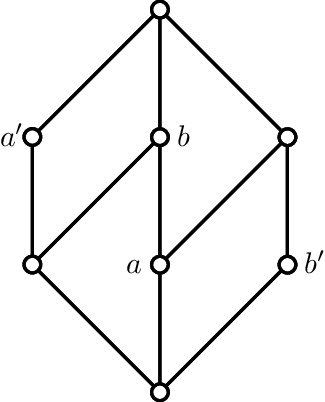
\includegraphics[scale=1]{compLattice}
\end{center}

By definition, $0$ is the common ancestor of all elements,
and $1$ the common successor of all elements. Inversely, all elements are
predecessors of $1$ and successors of $0$. Thus, if $1$ is a complement of some
element $a$, this element must be $0$, and vice-versa.

Given a bounded latice $(L, \lor, \land, 0, 1)$, we define $c : L \mapsto L $
as the unary \textit{complement} operation. Instead of writing $c(x)$ we shall
write $x^c$.

\begin{definition}
    A complemented lattice is a $6$-upla $(L, \lor, \land, ~^c, 0, 1)$ s.t.
    $(L, \lor, \land, 0, 1)$ is a bounded lattice and $~^c$ is a unary
    operation over $L$ s.t. $\forall x \in L :x \lor x^c = 1, x \land x^c = 0$.
\end{definition}

Note that is is possbile to define more than one unary operation that satisfies
the definition of complement.

\begin{problem}
    Consider the diamond poset $\left( \left\{ 1, 2, 3, 5, 30 \right\}, \mid
    \right) $. It clearly corresponds to bounded lattice in the algebraic
    sense. Find all unary operations $\lambda$ s.t. $(L, \lor, \land, \lambda,
    0, 1)$ is a complemented lattice.
\end{problem}


\small
\begin{quote}

    The image below depicts the diamond lattice, where the prime numbers 
    take the positions of $a, b, c$.

    \begin{center}
        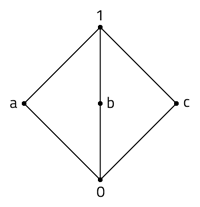
\includegraphics[scale=0.5]{diamond}
    \end{center}

    Observe that $a, b$  and $c$ are all complements of each other. Thus, any
    $\lambda$ s.t. $(L, \lor, \land, \lambda, 0, 1)$ is a complemented lattice
    must map each prime to either of the other two primes. Thus, 
    if we let $\mathcal{P} = \left\{ 2, 3, 5 \right\} $ the set of 
    primes in the lattice, the set of all complement functions is

    \begin{align*}
        \{ \lambda : L \to L \mid &~\lambda(0) = 1, \\ 
                                       &\lambda(1) = 0, \\ 
                                       &\forall p \in \mathcal{P} : \exists p' \in \mathcal{P} : p \neq p' \land  \lambda(p) = p' \}
    \end{align*}

    It is easy to observe that there are $2^3$ such functions, since we have
    $2$ options for each of the $3$ prime numbers.


\end{quote}
\normalsize

Let $(P, \leq)$ a poset with a maximum and minimum, and assume there is some
unary operation $\lambda : P \to P$ s.t. $\text{sup}\{x, \lambda(x)\}  = 1,
\text{inf}\{x, \lambda(x)\} = 0 $. Then defining $\lor$ and $\land$ as the
$\text{sup}$ and $\text{inf}$ functions of the poset satisfies that $(L, \lor,
\land, \lambda, 0, 1)$ is a complemented lattice.

Furthermore, by virtue of Dedekind's theorem, every complemented lattice is
obtained in this way. This entails that a poset with maximum, minimum and a
complement operation $\lambda$ is, in a certain sense, the same than its
corresponding complemented lattice.

\begin{tikzpicture}[remember picture, overlay, start chain, node distance=-2mm, shift={(-18mm, -12mm)}]
    \node [on chain]  {\pgfornament[width=1.72cm, color=darkscarlet]{158}};
\end{tikzpicture}
\subsection{Complemented sub-lattices}

\begin{definition}
    Given two complemented lattices $(L, \lor, \land, ~^c, 0, 1)$ and $(L',
    \lor', \land', ~^c', 0', 1')$, we say the first is a complemented
    sub-lattice of the latter iff

    \begin{itemize}
        \item $L \subseteq L  $
        \item $0 = 0', 1 = 1'$
        \item $\lor  = \lor'_{\mid L^2}, \land = \land'_{\mid L^2}, ~^c = ~^c_{\mid L}$
    \end{itemize}
\end{definition}

\begin{definition}
    Let $(L / \theta, \widetilde{\lor}, \widetilde{\land})$ a complemented
    lattice. A set $S \subseteq L$ is a sub-universe of the lattice if $\left\{
    0,1 \right\}\subseteq  S $ and $S$ is closed under $\land , \lor $ and
    $~^c$.
\end{definition}

As in previous cases, if $S$ is a sub-universe of $(L, \lor, \land, ~^c, 0,
1)$, then $(S, \lor_{| S^2}, \land_{|S^2}, ~^c_{|S^2}, 0, 1)$ is a complemented
sub-lattice of $(L, \lor, \land, ~^c, 0, 1)$, and every complemented
sub-lattice is obtained in this way. In other words, there is a bijection
between the set of complemented sub-lattice of $(L, \lor, \land, ~^c, 0, 1)$
and the set of sub-universes of $(L, \lor, \land, ~^c, 0, 1)$.

\begin{tikzpicture}[remember picture, overlay, start chain, node distance=-2mm, shift={(-18mm, -12mm)}]
    \node [on chain]  {\pgfornament[width=1.72cm, color=darkscarlet]{158}};
\end{tikzpicture}
\subsection{Homorphisms of complemented lattices}

\begin{definition}
    Let $(L, \lor, \land, ~^c, 0, 1), (L', \lor', \land', ~^c', 0', 1')$ two 
    complemented lattices. A function $F: L \mapsto  L'$ is a 
    homomorphism from the first to the latter if $\forall x, y \in L$:

    \begin{itemize}
        \item $F(x \circ y) = F(x) \circ' F(y)$.
        \item $F(x^c) = F(x)^{c'}$
        \item $F(0) = 0', F(1) = 1'$.
    \end{itemize}
\end{definition}

A homomorphism is an isomorphism if it is bijective and its inverse is 
a homorphism. In complemented sub-lattices, like all lattices so far, it
suffices to show that a homomorphism is bijective to prove that it's an
isomorphism. 

\begin{theorem}
    If $F : (L, \lor, \land, ~^c, 0, 1) \mapsto (L', \lor', \land', ~^c', 0', 1')$
    is a bijective homomorphism, then it is an isomorphism.
\end{theorem}


\small
\begin{quote}

\begin{pro}
    Analogous to previous cases.
\end{pro}

\end{quote}
\normalsize

\begin{theorem}
    If $F: (L, \lor, \land, ~^c, 0, 1)\mapsto (L', \lor', \land', ~^c', 0',
    1')$ is a homomorphism, then $I_F$ is a sub-universe of $(L', \lor',
    \land', ~^c', 0', 1')$. Which means $F$ is also a homomorphism from $(L,
    \lor, \land, ~^c, 0, 1)$ to $(I_F, \lor'_{|I_F^2}, \land'_{|I_F^2}, ^{c'},
    0', 1')$.
\end{theorem}


\small
\begin{quote}

\begin{pro}
    Analogous to previous cases.
\end{pro}

\end{quote}
\normalsize

\begin{tikzpicture}[remember picture, overlay, start chain, node distance=-2mm, shift={(-18mm, -12mm)}]
    \node [on chain]  {\pgfornament[width=1.72cm, color=darkscarlet]{158}};
\end{tikzpicture}
\subsection{Congruences over complemented lattices}

\begin{definition}
    A congruence over $(L, \lor, \land, ~^c, 0, 1)$ is an equivalence 
    relation $\theta$ s.t. $\theta$ is a congruence over 
    $(L, \lor, \land, 0, 1)$ and $x / \theta = y /\theta \Rightarrow x^c / \theta = y^c / \theta$.
\end{definition}

These conditions allow us to define $\widetilde{ \lor  } $ and $\widetilde{ \land  } $ in a fashion analogous to previous cases:

\begin{align*}
    &x / \theta ~ \widetilde{ \circ } y / \theta = (x \circ y) / \theta \\ 
    &(x / \theta)^{\widetilde{ c } } = x^c / \theta
\end{align*}

The $6$-uple $(L / \theta, \widetilde{\lor}, \widetilde{ \land}, ~^{\widetilde{
c }},  0 / \theta, 1/ \theta)$ is called the \textit{quotient space} of $(L,
\lor, \land, ~^c, 0, 1)$ over $\theta$ and we denote it as $(L, \lor, \land,
~^c, 0, 1) / \theta$.

\begin{theorem}
    If $(L, \lor, \land, ~^c, 0, 1)$ a complemented lattice and $\theta$ 
    a congruence over $(L, \lor, \land, ~^c, 0, 1)$:

    \begin{itemize}
        \item $(L / \theta, \widetilde{\lor}, \widetilde{ \land}, ~^{\widetilde{ c } }, 0 / \theta, 1/ \theta)$ is a complemented lattice. 
        \item $\pi_{\theta}$ is a homomorphism from $(L, \lor, \land, ~^c, 0, 1)$ to $(L / \theta, \widetilde{\lor}, \widetilde{ \land}, ~^{\widetilde{ c } } , 0 / \theta, 1/ \theta)$ and $\ker(\pi_\theta) = \theta$.
    \end{itemize}
\end{theorem}


\small
\begin{quote}

\begin{pro}
    (1) A previous theorem ensures that $(L / \theta, \widetilde{\lor},
    \widetilde{ \land}, 0 / \theta, 1/ \theta)$ is a bounded lattice, so we
    only to verify that the lattice identities hold for the $~^\widetilde{ c }
    $ operation.

    Let $x / \theta \in L / \theta$. By assumption $x \circ x^c = 1$, which entails 
    $(x \circ x^c) / \theta = 1/ \theta$. Then, by definition, 

    \begin{align*}
        &x / \theta \widetilde{ \circ  } (x^c) / \theta = 1/\theta \\ 
        \iff & x / \theta \widetilde{ \circ  } (x / \theta)^{\widetilde{ c } } = 1 / \theta
    \end{align*}

    (2) A previous theorem ensures that $\pi_{\theta}$ is a homorphism from 
    $(L, \lor, \land, 0, 1)$ to $(L / \theta, \widetilde{\lor}, \widetilde{
    \land}, 0 / \theta, 1/ \theta)$ whose kernel is $\theta$. We must only
    ensure that it satisfies the homorphism definition for the complement
    operation. 

    Let $x \in L$. We wish to prove $\pi_\theta(x^c) =
    \pi_\theta(x)^{\widetilde{ c }} $. By definition, 

    \begin{equation*}
        \pi_\theta(x)^{\widetilde{ c } } = \left( x / \theta \right)^{\widetilde{ c } } = (x^c) / \theta = \pi_\theta(x^c) ~ \blacksquare
    \end{equation*}



\end{pro}

\end{quote}
\normalsize

\begin{theorem}
    If $F : (L, \lor, \land, ~^c, 0, 1) \mapsto (L', \lor', \land', ~^c', 0',
    1')$ is a complemented lattice homomorphism, then $\ker(F)$
    is a congruence over $(L, \lor, \land, ~^c, 0, 1)$.
\end{theorem}

This is the analogue to \textbf{Theorem 17}, which stated this was the case for
general lattices.

\small
\begin{quote}

\begin{pro}



    Let $\lambda = \ker(F)$. By definition, $\lambda$ is a congruence over $(L,
    \lor, \land, 0, 1)$. Then all that remains to be shown is that $x / \lambda
    = y / \lambda \Rightarrow x^c / \lambda = y^c / \lambda$.

    Let $x, y \in L$ s.t. $x / \lambda = y / \lambda$. This entails 
    $F(x) = F(y)$. Since $F$ a homomorphism, 
    $F(x^c) = F(x)^c$, which entails 

    \begin{equation*}
        F(x)^c = F(y)^c \Rightarrow F(x^c) = F(y^c) \Rightarrow (x^c, y^c) \in \ker(F)
    \end{equation*}

    It follows directly that $x^c / \lambda = y^c / \lambda$. $\blacksquare$



\end{pro}

\end{quote}
\normalsize

\begin{tikzpicture}[remember picture, overlay, start chain, node distance=-2mm, shift={(-18mm, -12mm)}]
    \node [on chain]  {\pgfornament[width=1.72cm, color=darkscarlet]{158}};
\end{tikzpicture}
\subsection{A notational convention}

In the $n$-uples we have studied (posets and lattices of various kinds), the
first element of the $n$-uple was called its \textit{universe}. We shall use
bold letters to denote the universes of these structures. Thus, the phrase
"\textbf{L} is a bounded lattice" equates to saying $(L, \lor, \land, 0, 1)$ is
a bounded lattice.

Then writing that $F : \textbf{L} \mapsto L'$ is a homomorphism equates to
saying $F : (L, \lor, \land, 0, 1) \mapsto (L', \lor', \land', 0', 1')$ is a
homomorphism. Similarly, writing $\textbf{L} / \theta$, where $\theta$ a
congruence, will equate to writing the quotient space of whatever $n$-uple is
signified by \textbf{L}.

\pagebreak 

\begin{tikzpicture}[remember picture, overlay, start chain, node distance=-2mm, shift={(0mm, 10mm)}]
    \foreach \i in {1,...,3}
    \node [on chain]  {\pgfornament[width=6.72cm, color=darkscarlet]{71}};
\end{tikzpicture} 
\section{Boolean algebras} 

We have so far studied several kinds of mathematical structures
separately. In particular, we have studied different kinds of lattices,
observing a special property which defined them.

Now, we come to the study of structures which exhibit several of these
properties simultaneously. In particular, we will develop an understanding of
bounded and distributive lattices, show the connection of this combination with
complemented lattices, and from there develop the concept of a Boolean algebra.

\begin{definition}
    A bounded or complemented lattice \textbf{L} is said to be distributive 
    when $(L, \lor, \land)$ is distributive.
\end{definition}

Let $Dis_1$ denote distributivity of $\land $ with respect to $\lor $,
and $Dis_2$ the converse.

\begin{theorem}
    Let $(L, \lor, \land)$ a lattice. Then $(L, \lor, \land)$ satisfies 
    $Dis_1$ iff it satisfies $Dis_2$.
\end{theorem}


\small
\begin{quote}

\begin{pro}
    Assume $(L, \lor, \land)$ satisfies $Dis_1$. Let $a, b, c \in L$ fixed. 
    Then 

    \begin{equation*}
        (a \lor  b) \land  (a \lor  c) = \left( (a \lor  b) \land  a \right)  \lor  \left( (a \lor  b) \land  c \right) 
    \end{equation*}

    Commutativity then gives 

    \begin{equation*}
         \left( (a \lor  b) \land  a \right)  \lor  \left( (a \lor  b) \land  c \right) = (a \land (a \lor b)) \lor  (c \land  (a \lor  b))
    \end{equation*}


A funamental property of lattices is that $a \land (a \lor  b) = a$. Using 
this property with $Dis_1$,

\begin{equation*}
    (a \land (a \lor b)) \lor  (c \land  (a \lor  b)) = a \lor \left( (c \land  a) \lor  (c \land  b) \right) 
\end{equation*}

Due to the associative property, 

\begin{equation*}
    = a \lor \left( (c \land  a) \lor  (c \land  b) \right) = \left( a \lor (c \land a) \right) \lor (c \land b)
\end{equation*}

Commutativity gives

\begin{equation*}
    \left( a \lor (c \land a) \right) \lor (c \land b) = (a \lor  (a \land  c)) \lor (b \land  c) = a \lor (b \land  c)
\end{equation*}

Then we have proven $a \lor (b \land  c) = (a \lor  b) \land  (a \lor c)$. $\blacksquare$.

The other direction of the double implication is analogous.

\end{pro}

\end{quote}
\normalsize

\begin{definition}
    A Boolean algebra is a complemented lattice $\textbf{L}$ that is distributive.
\end{definition}

\begin{theorem}
    Let $\textbf{L}$ a bounded lattice that is distributive. Then every element 
    has at most one complement.
\end{theorem}


\small
\begin{quote}

\begin{pro}
    Let $x, y, z \in L$ fixed. Assume $x \lor  y = x \lor  z = 1$ 
    and $x \land  y = x \land  z = 0$. Observe that 
    $y = y \land  1 = y \land (x \lor  z)$. Because $\textbf{L}$ is 
    distributive, we have $y = (y \land  x) \lor  (y \land  z)$.
    Then $y = 0 \lor  (y \land   z) = y \land  z$.

    The same line of reasoning gives $z = z \land  1 = z \land  (x \lor  y)$, from
    which follows $z = (z \land  x) \lor  (z \land  y) = z \land  y$.

    $\therefore $ $z = z \land  y = y \land  z = y$.

    $\therefore $ $z = y$.
\end{pro}

\end{quote}
\normalsize

\begin{theorem}
    Let $(B, \lor , \land , ~^c, 0, 1)$ a Boolean algebra. For any $x, y \in B$,
    $y = (y \land  x) \lor  (y \land x^c)$.
\end{theorem}


\small
\begin{quote}

\begin{pro}
    Let $x, y \in B$. Then

    \begin{align*}
        (y \land  x) \lor  (y \land x^c) &= \left[ (y\land x) \lor  y \right] \land \left[ (y \land  x) \lor  x^c \right] &\left\{ \text{Dist.} \right\} \\ 
                                         &=\left[ (y \lor  y) \land  (y \lor  x) \right] \land \left[ (y \lor x^c) \land (x \lor  x^c) \right] &\left\{ \text{Dist.} \right\} \\ 
                                         &=\left[ y \land (y \lor  x) \right] \land \left[ (y \lor  x^c) \land 1 \right] &\left\{ \text{Comp., abs.} \right\} \\ 
            &= y \land (y \lor  x^c) \\ 
            &=y
    \end{align*}

    where the last two steps use the property $y \land (y\lor x) = y$.

\end{pro}

\end{quote}
\normalsize

\begin{theorem}
    Let $\textbf{B}$ a Boolean algebra and $x, y \in B$. Then: 

    \begin{itemize}
        \item $(x \land y)^c = x^c \lor  y^c$ ~ ~ ~ (DeMorgan's law 1)
        \item $(x \lor  y)^c = x^c \land   y^c$ ~ ~ ~ (DeMorgan's law 2)
        \item $(x^c)^c = x$
        \item $x \land  y = 0 \iff y \leq x^c$
        \item $x \leq y \iff y^c \leq x^c$
    \end{itemize}
\end{theorem}

If one thinks of the associated posset, the proposition $x \land  y = 0$  may
be read as "$y$ is not an ancestor of $x$". Thus, the fourth property states 
if $y$ is not an ancestor of $x$, then it must be an ancestor of $x^c$.

Similarly, the last property states that if $x$ is an ancestor of $y$,
$y^c$ is an ancestor of $x^c$.


\small
\begin{quote}

\begin{pro}
    We will prove the fourth and fifth properties. 

    \textit{(Property 4)} Assume $x \land  y = 0$. The previous 
    theorem gives

    \begin{align*}
        y &= (y \land  x) \lor  (y \land x^c)\\ 
          &= y \land x^c
    \end{align*}

    $\therefore $ $y \leq x^c$.

    Now assume $y \leq x^c$. Then $y \land  x \leq x^c \land x$. 

    $\therefore $ $y \land  x \leq 0$. 

    $\therefore $ $y \land  x = 0$.

    \textit{(Property 5)} Assume $x \leq y$. Then $(x \land  y) = x$. Then $(x
    \land  y)^c = x^c$, and $x^c \lor y^c = x^c$. Then $x^c \land  y^c = y^c$
    and $y^c \leq x^c$.

    Now assume $y^c \leq x^c$. Then $(y^c \land x^c) = y^c$. Then $(y^c)^c \lor
    (x^c)^c = (y^c)^c$, which entails $y \lor  x = y$. Then $x \leq y$.

    $\blacksquare$


\end{pro}

\end{quote}
\normalsize

\begin{problem}
    Due the properties of the previous theorem hold for any complemented 
    lattice?
\end{problem}


\small
\begin{quote}

The answer is no; we need distributivity. But prove it. Complete.

\end{quote}
\normalsize


\begin{tikzpicture}[remember picture, overlay, start chain, node distance=-2mm, shift={(-18mm, -12mm)}]
    \node [on chain]  {\pgfornament[width=1.72cm, color=darkscarlet]{158}};
\end{tikzpicture}
\subsection{Prime filters and Rasiova-Sikorski's theorem}

\begin{definition}
    A filter of a lattice $(L, \lor, \land)$ will be any non-empty subset $F \subseteq L$ s.t. 

    \begin{itemize}
        \item $x, y \in F \Rightarrow x \land y \in F$ 
        \item $x \in F$ and $x \leq y \Rightarrowy \in F$
    \end{itemize}
\end{definition}

\begin{problem}
    Describe the filters of $(\mathbb{R}, \max, \min)$. For any given filter, 
    does it always contain an infimum?
\end{problem}


\small
\begin{quote}

    Observe that $(\mathbb{R}, \max, \min)$ induces via Dedekind's theorem the
    totally ordered set $(\mathbb{R}, \leq)$, where $\leq$ is the usual order.
    Consider any filter $F \subseteq \mathbb{R}$. The inclusion of any element
    in $F$ implies the inclusion of all numbers greater than that element.
    Thus, the filters of $(\mathbb{R}, \max, \min)$ consists of all 
    continuous subsets of $\mathbb{R}$; i.e. 

    \begin{equation*}
        \text{Set of filters of $(\mathbb{R}, \max, \min)$} = \left\{ [x, \infty) : x \in \mathbb{R} \right\} 
    \end{equation*}

    Clearly, since any filter is of the form $[x, \infty)$ with $x \in
    \mathbb{R}$, $x$ is always the infimum of that filter.

\end{quote}
\normalsize

\begin{problem}
    Find all filters of $\left( \left\{ 1, 2, 3, 6, 12 \right\}, \lcm, \gcd  \right) $.
\end{problem}


\small
\begin{quote}


Evidently, $\left\{ 1, 2, 3, 6, 12 \right\} $ is a filter, 
and is the only filter which contains $1$.

Consider a filter which contains $2$. If it contains $3$ it must contain $1$
and we are back in the first case. So $\left\{ 2, 6, 12 \right\} $ is a filter.
A similar argument leads to $\left\{ 3, 6, 12 \right\} $.

Lastly, $\left\{ 6, 12 \right\} $ and $\left\{ 12 \right\} $ are filters.

\end{quote}
\normalsize

Let us present some notation. Given $S \subseteq L$, we use $[S)$ to 
denote the set 

\begin{equation*}
    \left\{ x \in L : y \geq (s_1 \land  \ldots \land s_n) \text{ for some } s_1, \ldots, s_n \in S, n \geq 1 \right\} 
\end{equation*}

and we call it the filter \textit{generated} by $S$.

The set $[S)$ is clearly a subset of $L$. If $l \in L$ is a successor of any
element of $S$, or of the infimum between any set of elements in $S$, then $l
\in [S)$. In a certain sense, the elements of $[S)$ are the successors of all
elements of $S$ or some of their predecessors.

Since any element in $S$ is a successor to itself, all elements of $S$ are in
$[S)$. In other words, $S \subseteq [S) \subseteq L$.

When $S$ is finite, $[S) = \left\{ y \in L : y \geq \text{inf}(S) \right\} $.
When $S$ is infinite but has an infimum, in many cases the statement will hold
as well, but there are exceptions.

\begin{example}
    Let $\textbf{L} = \left( \mathcal{P}(\mathbb{N}), \cup, \cap  \right) $ and 
    $S = \left\{ \mathbb{N} - n : n \in \mathbb{N} \right\} $. 
    The infimum of $S$ is $\emptyset$ and $[S) = \left\{ A \in
    \mathcal{P}(\mathbb{N}) : \mathbb{N} - A \text{ is finite}\right\} $.

    Then it doesn't hold that $[S) = \left\{ y \in L : y \geq \text{inf} S
    \right\} $.
\end{example}

\begin{theorem}
    Assume $S$ is non-empty. Then $[S)$ is a filter. Furthermore, if $F$ a
    filter and $S \subseteq F$, then $[S) \subseteq F$. In other words, $[S)$
    is the minimal filter which contains $S$.
\end{theorem}


\small
\begin{quote}

\begin{pro}
    Since $S \subseteq [S)$ we have $[S) \neq \emptyset$. It is trivial to observe 
    that $[S)$ satisfies that if an element is in $[S)$, all 
    its successors will also be in $[S)$. Let us show that 
    the infimum of any pair in $[S)$ is also in $[S)$.

    Assume $x, y \in [S)$. Then $x \geq s_1 \land  \ldots \land  s_n$ and $y
    \geq t_1\land \ldots \land  t_m$ for $n, m \geq 1$ and $s_j, t_j \in S$.
    Then 

    \begin{equation*}
        x \land  y \geq (s_1 \land  \ldots \land s_n) \land (t_1 \land  \ldots t_m)
    \end{equation*}

    which completes the proof.
\end{pro}

\end{quote}
\normalsize

\begin{definition}
    Let $(P, \leq)$ a poset. A subset $C \subseteq P$ is a chain if for every
    $x, in \in C$, $x \leq y$ or $y \leq x$.
\end{definition}

Chains may be infinite and given an infinite chain $C$, there may not exist an
infinite sequence $\left\{ c_1, c_2, \ldots \right\} $ s.t. $C = \left\{ c_n :
n \in \mathbb{N} \right\} $.

\begin{example}
    Every subset of $\mathbb{R}$ is a chain of $(\mathbb{R}, \leq)$. Observe
    that there is no discrete infinite sequence $c_1, c_2,\ldots$ which may
    account for a subset of $\mathbb{R}$.
\end{example}


\begin{theorem}[Zorn's theorem]
    Let $(P, \leq) $ a poset and assume every chain of $(P, \leq) $ has an
    upper bound. Then there is a maximal element in $(P, \leq) $.
\end{theorem}


\small
\begin{quote}

\begin{pro}
    Complete.
\end{pro}

\end{quote}
\normalsize

\begin{definition}[Prime filter]
    A filter $F$ on a lattice $(L, \lor, \land)$ is called \textit{prime} when
    $F \neq L$ and $x \lor  y \in F \Rightarrow x \in F \lor  y \in F$.
\end{definition}

\begin{problem}
    Show that every filter of $(\mathbb{R}, \max, \min)$ other than $\mathbb{R}$
    is prime.
\end{problem}


\small
\begin{quote}

    The lattice $\textbf{L} = (\mathbb{R}, \max, \min)$ induces the total order
    $(\mathbb{R}, \leq)$. Let $\mathcal{F}$ an arbitrary filter of \textbf{L}
    different from $\mathbb{R}$. Assume $x \max y \in \mathcal{F}$ for $x, y
    \in \mathbb{R}$. Since $x \max y \in \left\{ x, y \right\} $, either $x \in
    \mathcal{F}$ or $y \in \mathcal{F}$. Then $\mathcal{F}$ is prime.
    $\blacksquare$

\end{quote}
\normalsize

\begin{problem}
    Find all prime filters over $\textbf{L} = \left( \left\{ 1, 2, 3, 6, 12 \right\}, \lcm, \gcd  \right) $.
\end{problem}


\small
\begin{quote}

    In \textbf{Problem 48} we found all filters of \textbf{L}. The question is
    which, except for $L$, were prime? 

    Clearly, $\left\{ 6, 12 \right\} $ is not prime, because $6 = 3 \lor 2$ and
    it doesn't contain either $3$ nor $2$. Same observation 
    yields that $\left\{ 2, 6, 12 \right\} $ and $\left\{ 3, 6, 12
    \right\} $ are prime. Finally, $\left\{ 12 \right\} $ is trivially prime:
    $12 \lor  12 = 12$.


\end{quote}
\normalsize

\begin{theorem}[Prime filter theorem]
    Let $\textbf{L}$ a distributive lattice and $F$ a filter of $\textbf{L}$.
    Assume $x_0 \in L - F$. Then there is a prime filter $P$ s.t. 
    $x_0 \not\in P$ and $F \subseteq P$.
\end{theorem}


\small
\begin{quote}

\begin{pro}
    Let 

    \begin{equation*}
        \mathcal{F} := \left\{ F_1 : F_1 \text{ is a filter}, x_0 \not\in F_1,F \subseteq F_1 \right\} 
    \end{equation*}

    Since $F \in \mathcal{F}$, $\mathcal{F} \neq \emptyset$ and $\textbf{F} = (\mathcal{F}, \subseteq )$ 
    is a poset. Let us prove that every chain in the poset 
    has an upper bound.

    Let $C$ a chain over $\textbf{F}$. If $C = \emptyset$, every 
    element in $\mathcal{F}$ is an upper bound. If $C \neq \emptyset$,
    we can define 

    \begin{equation*}
        G = \left\{ x \in L : x \in F_1 \text{ for some } F_1 \in C \right\} 
    \end{equation*}

    It is clear that $G \neq \emptyset$. Assume $x, y \in G$. Let $F_1, F_2 \in
    \mathcal{F}$ s.t. $x \in F_1$ and $y \in F_2$.

    If $F_1 \subseteq F_2$, since $F_2$ a filter we have $x \land  y \in F_2
    \subseteq G$. If $F_2 \subseteq F_1$ then $x\land  y \in F_1 \subseteq G$.
    Since $C$ a chain $x \land  y \in G$. The remaining 
    property is proved in analogous fashion.

    $\therefore $ $G$ is a filter. 

    Since $x_0 \not\in G$ we know $G \in \mathcal{F}$ is upper-bound of $C$.
    Due to Zorn's theorem, $(\mathcal{F},\subseteq )$ has a maximal element
    $\mathcal{M}$. We shall show $\mathcal{M}$ is prime.

    Assume $x \lor  y \in \mathcal{M}$ and $x, y \not\in \mathcal{M}$.
    Observe that $[\mathcal{M} \cup \left\{ x \right\}) $ is a filter 
    which properly contains $\mathcal{M}$. Since $\mathcal{M}$
    is maximal of $(\mathcal{F}, \subseteq)$ we have $x_0 \in [\mathcal{M} \cup \left\{ x \right\}) $.
    Analogously, $x_0 \in [\mathcal{M} \cup \left\{ y \right\} )$. 
    
    Since $x_0 \in [\mathcal{M} \cup \left\{ x \right\}) $ there 
    are $m_1, \ldots, m_n \in \mathcal{M}$ s.t. 

    \begin{equation*}
        x_0 \geq m_1 \land  \ldots \land  m_n \land  x
    \end{equation*}

    Since $x_0 \in [\mathcal{M}, \left\{ y \right\}) $ there are 
    $m'_1, \ldots, m'_r \in \mathcal{M}$ s.t. 

    \begin{equation*}
        x_0 \geq m_1' \land  \ldots m_r' \land  y
    \end{equation*}

    Let $m := m_1 \land  \ldots \land  m_n \land  m_1' \land  \ldots \land  m_r'$.
    Then we have $x_0 \geq m \land  x$ and $x_0 \geq m \land  y$.

    $\therefore $ $x_0 \geq (m \land  x) \lor  (m \land  y) = m\land (x \lor  y)$.

    But this is absurd because $x_0 \not\in \mathcal{M}$. The contradiction 
    ensued from assuming $x, y \not\in \mathcal{M}$.

    $\therefore $ Either $x \in \mathcal{M}$ or $y \in \mathcal{M}$.

    $\therefore $ $\mathcal{M}$ is prime.
    


\end{pro}

\end{quote}
\normalsize

Let us unpack the theorem. Assume $\textbf{L}$ is a distributive lattice 
and $F$ is a filter over it. Assume as well that some $x_0 \in L$ is not 
contained in the filter. We are interested in the family $\mathcal{F}$ of filters which do not contain
$x_0$ and contain all elements of $F$. Informally, we may call these
\textit{extensions of $F$ around $x_0$}. Such family conforms a poset
$(\mathcal{F}, \subseteq )$. The theorem states that \textit{(1)} this poset
has a maximal element and \textit{(2)} it is a prime filter.

\begin{theorem}[Rasiova-Sikorski's]
    Let $\textbf{B}$ a Boolean algebra. Let $\varphi \in B$ a non-zero element. Assume $(A_1, A_2, \ldots )$
    is an infinituple of subsets of $B$ s.t. each subset has an infimum. Then there is a 
    prime filter $P$ which satisfies: 

    \begin{itemize}
        \item $\varphi \in P$
        \item $\forall j \in \mathbb{N} : A_j \subseteq P \Rightarrow \text{inf}(A_j) \in P$
    \end{itemize}
\end{theorem}


\small
\begin{quote}

\begin{pro}
    It is accepted without proof.
\end{pro}

\end{quote}
\normalsize


\pagebreak 

\begin{tikzpicture}[remember picture, overlay, start chain, node distance=-2mm, shift={(0mm, 10mm)}]
    \foreach \i in {1,...,3}
    \node [on chain]  {\pgfornament[width=6.72cm, color=darkscarlet]{71}};
\end{tikzpicture}
\section{Structures and their associated languages}

We have so far studied several kinds of structures. We begain with posets and
noted that they were, in a certain sense, equivalent to algebraic lattices. We 
studied different families of lattices, which are schematized in the diagram 
below.

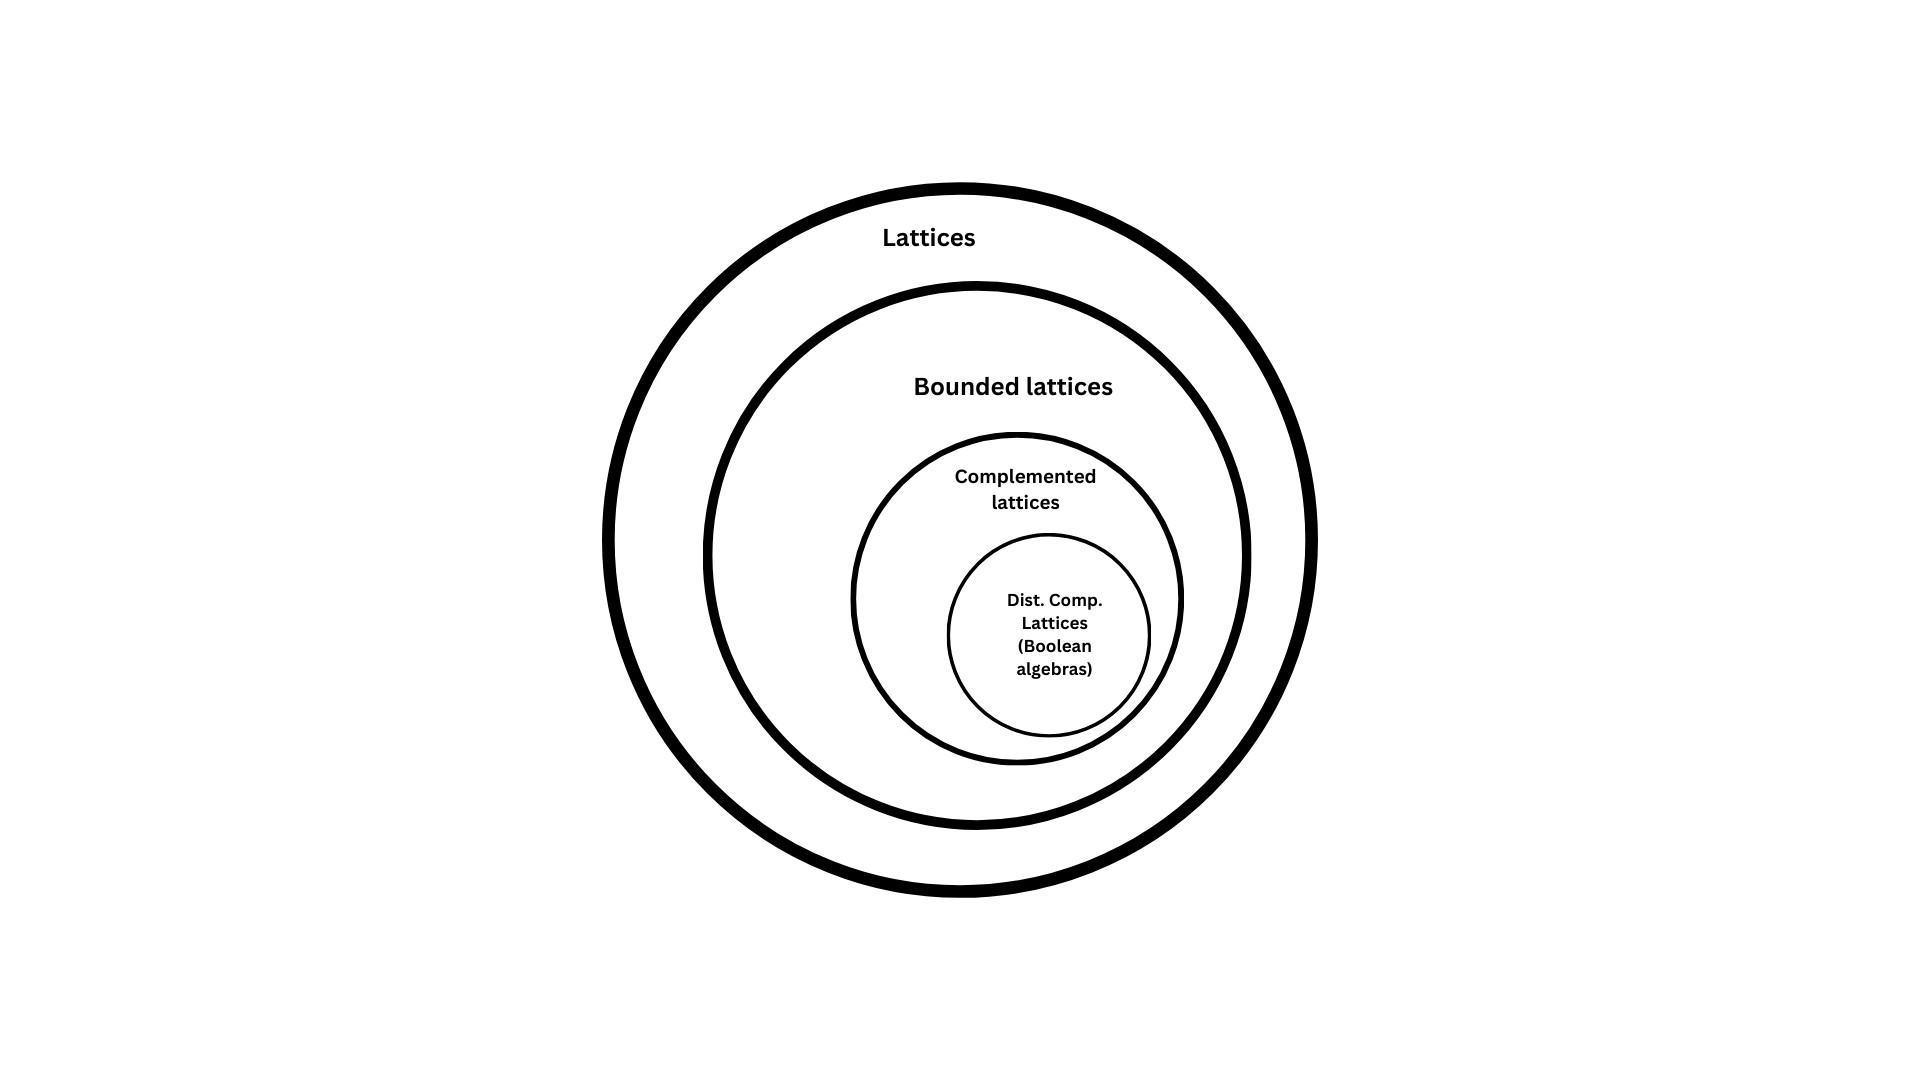
\includegraphics[scale=0.35]{latticeRings}

We will associate to each structure a set of sentences which we call
\textit{elementary formulas}. These formulas will serve as axioms to, in turn,
conform another type of sentence termed \textit{elementary proofs}. It is
important to observe that these sentences are relative to the particular kind of
structure that is being considered.

Elementary formulas will be formed with the usual symbols $\forall , \exists , \neg, \land , \ldots$ 
etc. We use $x, y, z,\ldots$ to denote variables and $a, b, c, \ldots$ to denote 
fixed elements. For instance, 

\begin{equation*}
    \neg\exists y \left( x \leq y \land \neg(y = x)  \right) 
\end{equation*}

is an elementary formula. Importantly, if $\varphi$ is a formula, then the type
of $\varphi$ is \textbf{word}.

A formula will be true or false depending on a particular poset $(P, \leq) $.
The variables of the formula will receive their values from said poset. When 
the formula has no free variables, we say it is an \textit{elementary poset sentence}.
Furthermore, as a convention, the quantifiers $\forall $ and $\exists $ always 
range over $P$. To keep matters clear, we will never quantify over fixed elements;
i.e. $\forall a(a=x)$ is not an elementary formula. 


\begin{example}
    Let $\textbf{P} = (\mathbb{N}, \mid)$. The formula $(x \leq y)$ is true when 
    $x$ is assigned $6$ and $y$ $36$. But the formula $\forall x \forall y\left( x \leq y \lor y \eq x \right) $ is false.
\end{example}

\begin{tikzpicture}[remember picture, overlay, start chain, node distance=-2mm, shift={(-18mm, -12mm)}]
    \node [on chain]  {\pgfornament[width=1.72cm, color=darkscarlet]{158}};
\end{tikzpicture}
\subsection{Free variables}















\end{document}



